\section*{Preface}
In this chapter, we discuss the performance of AIBs using carbonised natural products (such as human hair, hemp fibers) and a few other carbon-based materials as cathodes and try to establish their mechanism.
\pagebreak
\chapter{Carbon-based cathodes for rechargeable AIBs} % Main chapter title

\label{chap5} % For referencing the chapter elsewhere, use \ref{Chapter1} 

%----------------------------------------------------------------------------------------
% Define some commands to keep the formatting separated from the content 
%Different forms of carbon: activated carbon from human hair (ACH), hemp fibers, a fullerene extract (CFEx) and Super-P carbon black were tested as cathodes for non-aqueous aluminium-ion batteries. These materials differ in their general structure, porosity and morphology. The fullerenes display a crystalline structure, whereas hemp fibers, Super-P and ACH are amorphous in nature. Of all materials, ACH recorded the highest specific capacity after 50 cycles at 103 mAh g$^{-1}$ with a coulombic efficiency of ~90\% at a current rate of 50 mV s$^{-1}$. Both hemp fibers and SPC achieved their highest specific capacities at 56 mAh g-1 and 84 mAh g$^{-1}$ respectively. CFEx, a mixture of \ce{C60} (85\%) and \ce{C70} (15\%) fullerene, recorded its highest capacity at 78 mAh g$^{-1}$ and maintained it for 50 cycles. The cells were charged and discharged to 2.45 V and 0.2 V respectively. 

\section{Theory and background}
Different varieties of carbon-based materials have been widely used in energy storage applications. Activated carbons are the most widely used materials today, because of their high specific surface area and low cost. They are derived by carbonisation (heat treatment) of carbon-rich compounds in inert atmosphere. Precursors can range from natural materials, such as human hair, rice husk, coconut shells, wood, or synthetic materials, such as polymers. A porous network in the bulk of the carbon particles is produced after activation; micropores (<2 nm in size), mesopores (2–50 nm) and macropores (>50 nm) can be created in carbon grains. Accordingly, the porous structure of carbon is characterized by a broad distribution of pore size. Longer activation time or higher temperature leads to larger mean pore size \cite{simon_materials_2008}. In 2000, Sony commercialised LIBs, where metallic lithium was replaced by a carbon host structure that reversibly absorbed and released \ce{Li+} ions at low electrochemical potentials \cite{ozawa_lithium-ion_1994}. The need for carbon was to allow high capacity for reversible lithium-ion absorption at a potential close to lithium metal. This was a major breakthrough, and was immediately followed by all major battery manufacturers. Researchers coined the term 'rocking-chair' for the  continuous intercalation/ deintercalation of ions from one electrode to the other during charge/ discharge cycles in these battery systems. After Sony, a large variety of carbons with low crystallinity were tested as electrode materials. They revealed very different electrochemical behaviours due to their different micro and macroscopic structures. In most of the LIBS we use today, lithiated carbon (\ce{LiC6}) is used as an anode and a lithium metal oxide acts as the cathode (\ce{LiCoO2}, \ce{LiNiO2}, \ce{LiMn2O4}).   
%In early attempts, graphite could not be used as an anode because it reacted strongly with the electrolyte (6,7). Armand \textit{et al.} in the 1980's found out that lithiated carbon was a suitable alternative.  

\begin{table}
\caption{Characteristics of commonly used rechargeable batteries.} \label{table2xps}
\begin{center}
\begin{tabular}{ |p{0.5cm}|p{2.5cm}|p{2cm}|p{2.5cm}|p{2.5cm}|p{1.5cm}|}
\hline
\textbf{Ref} & \textbf{Cathode} & \textbf{Electrolyte} & \textbf{Specific capacity (mAh g$^{-1}$)} & \textbf{Current rate (mA g$^{-1}$)} & \textbf{No. of cycles} \\
\hline
\cite{wang_advanced_2017} & Natural graphite & EMImCl & 60 & 100 & 6000 \\
\cite{song_long-life_2017} & Graphite & NaCl & 43 & 100 & 9000 \\
\cite{sun_new_2015} & Carbon paper & EMImCl & 63 & 50 & 50+ \\
\cite{lin_ultrafast_2015-3} & 3D graphite foam & EMImCl & 70 & 4000 & 7500 \\
\cite{rani_fluorinated_2013} & Fluorinated natural graphite & DiBIMCl & 225 & 60 & 40 \\
\cite{stadie_zeolite-templated_2017} & Zeolite template carbon & EMImCl & 60 & 100 & 50+ \\
& Graphite & EMImCl & 116 & 5000 & 50+ \\

\hline
\end{tabular}
\end{center}
\end{table}

Graphite is a naturally occurring crystalline form of carbon and is found in abundance in many places around the world. As a result, the cost of raw graphite remains low. It has been used as an electrode in other battery systems as well. It has a layered structure, and a good thermal and electrical conductivity. It turned out to be an ideal intercalation electrode material in LIBs \cite{ji_recent_2011, yoo_large_2008, lian_large_2010}. For low cost aluminium battery systems, a graphite electrode could be appealing. Studies reveal that reversible ion intercalation into graphite is responsible for the storage capacities in AIBs \cite{rani_fluorinated_2013-1, lin_ultrafast_2015-3}. \ce{AlCl4-} anions intercalate into the graphitic layers when the cell is being charged and deintercalate during discharge. Different forms of graphite such as fluorinated graphite, kish graphite flakes, three-dimensional graphitic-foam, graphene aerogels and several other forms have been tested as cathodes for AIBs, which showed specific capacities ranging from 60-250 mAh g$^{-1}$ \cite{rani_fluorinated_2013-1, wang_kish_2017-1, wu_3d_2016, huang_graphene_2019}. Post mortem analysis of the cathodes in charged / discharged state revealed the intercalation/ deintercalation of \ce{AlCl4-} in the graphene layers. For example, \textit{ex- situ} X-ray diffraction patterns of a charged graphite cathode displayed the disappearance of the sharp graphitic (002) peak at 2$\theta$ = 26.55$^{\circ}$. Two new peaks emerged at 28.25$^{\circ}$ and 23.56$^{\circ}$. The peak separation suggested expansion of the graphitic host layers to 5.7\AA. Since the size of \ce{AlCl4-} anions is 5.28\AA, it confirmed the intercalation of \ce{AlCl4-} anions into the cathode \cite{lin_ultrafast_2015-3, wang_kish_2017-1}. To further reduce the cost of AIBs, we prepared carbonised natural products and tested them as cathodes for rechargeable AIBs. 

%Activated carbon, owing to its porous structure, provides a high surface area for absorption of electrolyte ions in super-capacitors \cite{eliad_ion_2001, zhu_carbon-based_2011-2}. X-ray diffraction (XRD) and Raman spectroscopy studies have widely been used to establish this mechanism \cite{rani_fluorinated_2013, wang_advanced_2017, lin_ultrafast_2015-3} as shown in Figure \ref{Figures/chap5fig:graphmech}. XPS studies have confirmed reversible oxidation/reduction of carbon when \ce{AlCl4-} anions intercalate/deintercalate respectively \cite{stadie_zeolite-templated_2017, liu_binder-free_2019}.

%Graphene, discovered in 2004, has very high crystallinity. Its one of the thinnest and strongest materials known to mankind. It is basically a 2D crystal with monolayers of carbon atoms arranged in a honeycomb structure with a 6-membered ring. Graphene, building block of graphite, has the maximum surface area to volume ratio in layered materials.

 \begin{figure}[tbh!]
  \centering
  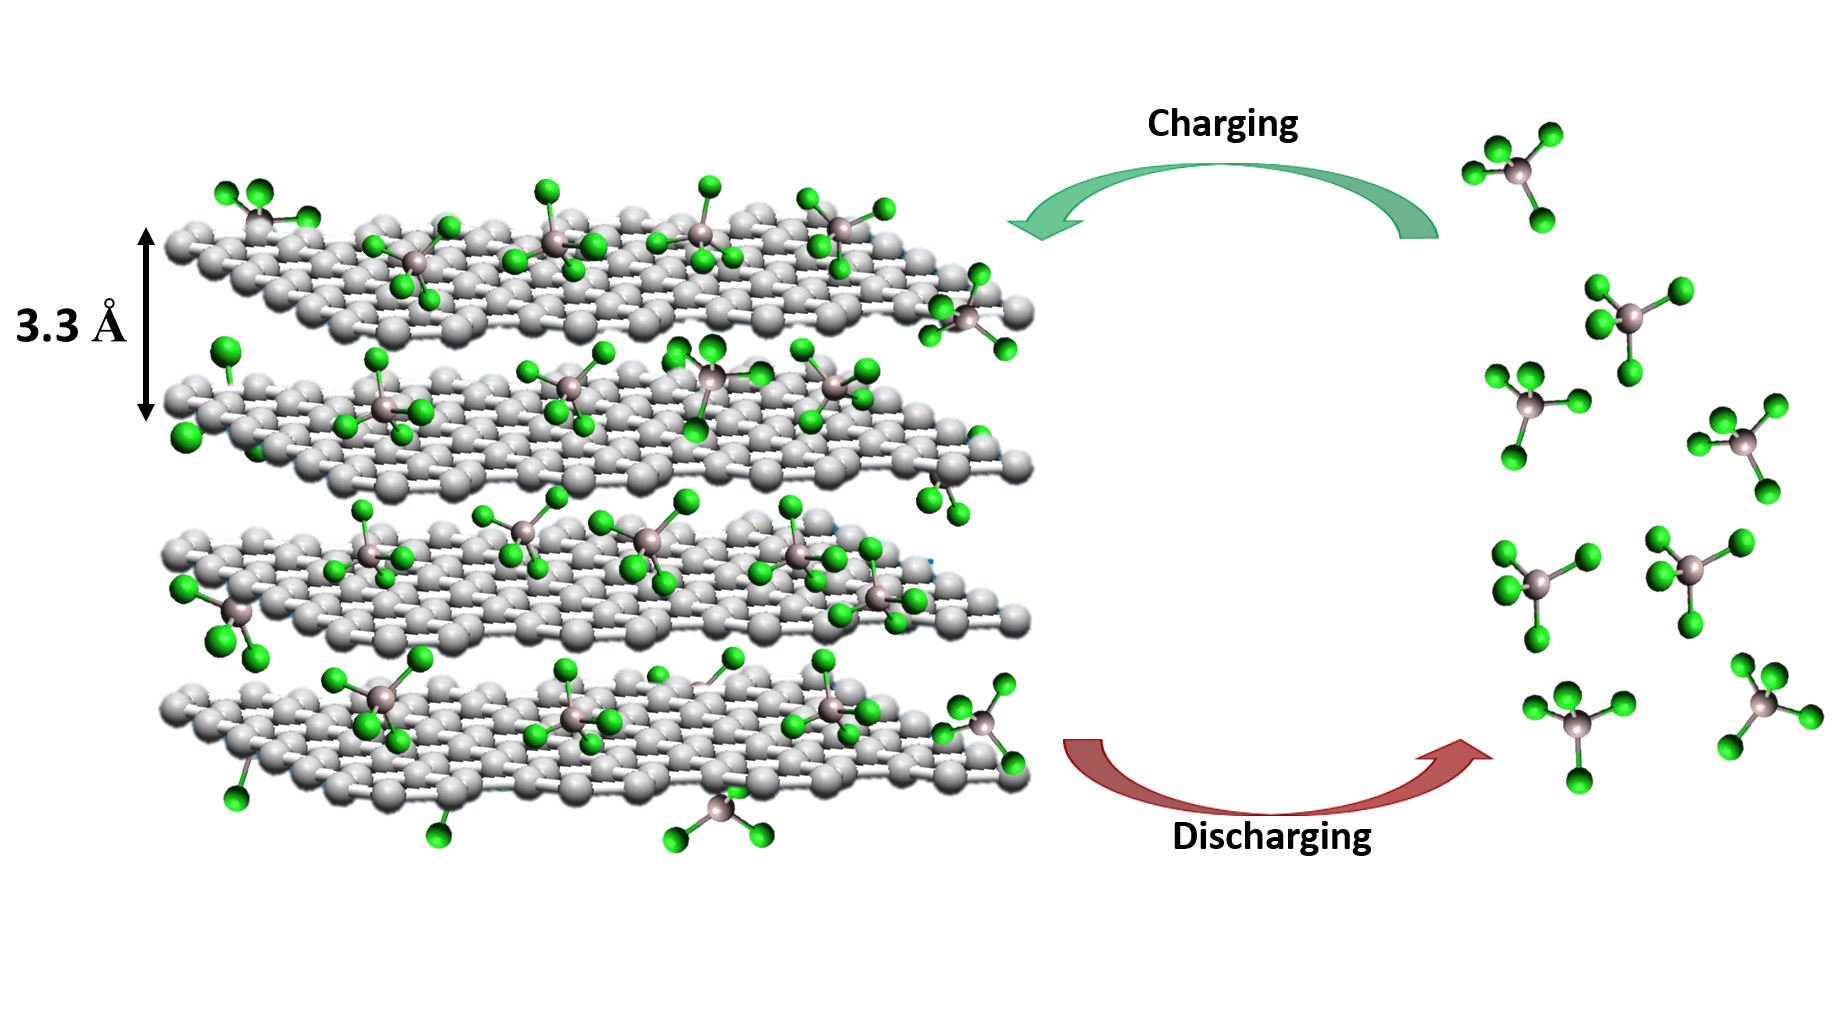
\includegraphics[width=\textwidth]{Figures/chap5fig/graphmech}
    \caption{Intercalation of \ce{AlCl4-} ions during cell charge and deintercalation during discharge in a Al/graphite cell. The interlayer distance between two graphite sheets is 3.3 \AA.}
  \label{Figures/chap5fig:graphmech}
\end{figure}

We compared four different carbon-based materials- activated carbon from human hair, activated carbon from hemp fibers, fullerenes and Super-P carbon black. Super-P carbon black is an amorphous form of carbon. It is highly conductive and is added in electrode slurries to enhance the conductivity of a cathode material. Activated carbon, also known as 'hierarchical porous carbons', derived from natural products such as rice husk, coconut shells or wood, have been previously used in batteries and super-capacitors \cite{hussain_development_2019, frackowiak_carbon_2001}. These structures contain pores of various sizes (mesopores and micropores). Mixture of \ce{C60} and \ce{C70} fullerenes was also tried as a cathode material. Fullerenes have a cage-like structure that gives them a very high surface area. Materials with high surface area adsorb ions on the surface of the material reversibly or sometimes undergo fast surface redox reactions. Based on these analogies, we tried  

\section{Results and discussion}

\begin{table}[h!]
\caption{Comparing battery metrics of all carbon-based cathodes tested in this work} \label{table1bm}
\begin{center}
\begin{tabular}{|lcccc|}
\hline
Active material & {\textbf{Size}} & {\textbf{Specific capacity}} & {\textbf{Cell efficiency}} & {\textbf{Cell voltage}}\\
 & {\textbf{(pore size)}} & {\textbf{(mAh g$^{-1}$)}} & {\textbf{(\%)}} & {\textbf{(V)}}\\
\hline
Human hair & 5${\mu}$ m & 102 & 97 & 1.9 \\
Fullerene mix & 8.8 \AA & 78 & 85 & 1.7 \\
Hemp fibers & 2.3 $\mu$ m & 49 & 75 & 1.8 \\
SPCB & 300 \AA & 46 & 40 & 1.5 \\
\hline  % Please only put a hline at the end of the table
\end{tabular}
\end{center}
\end{table}

\begin{figure}[h!]
  \centering
  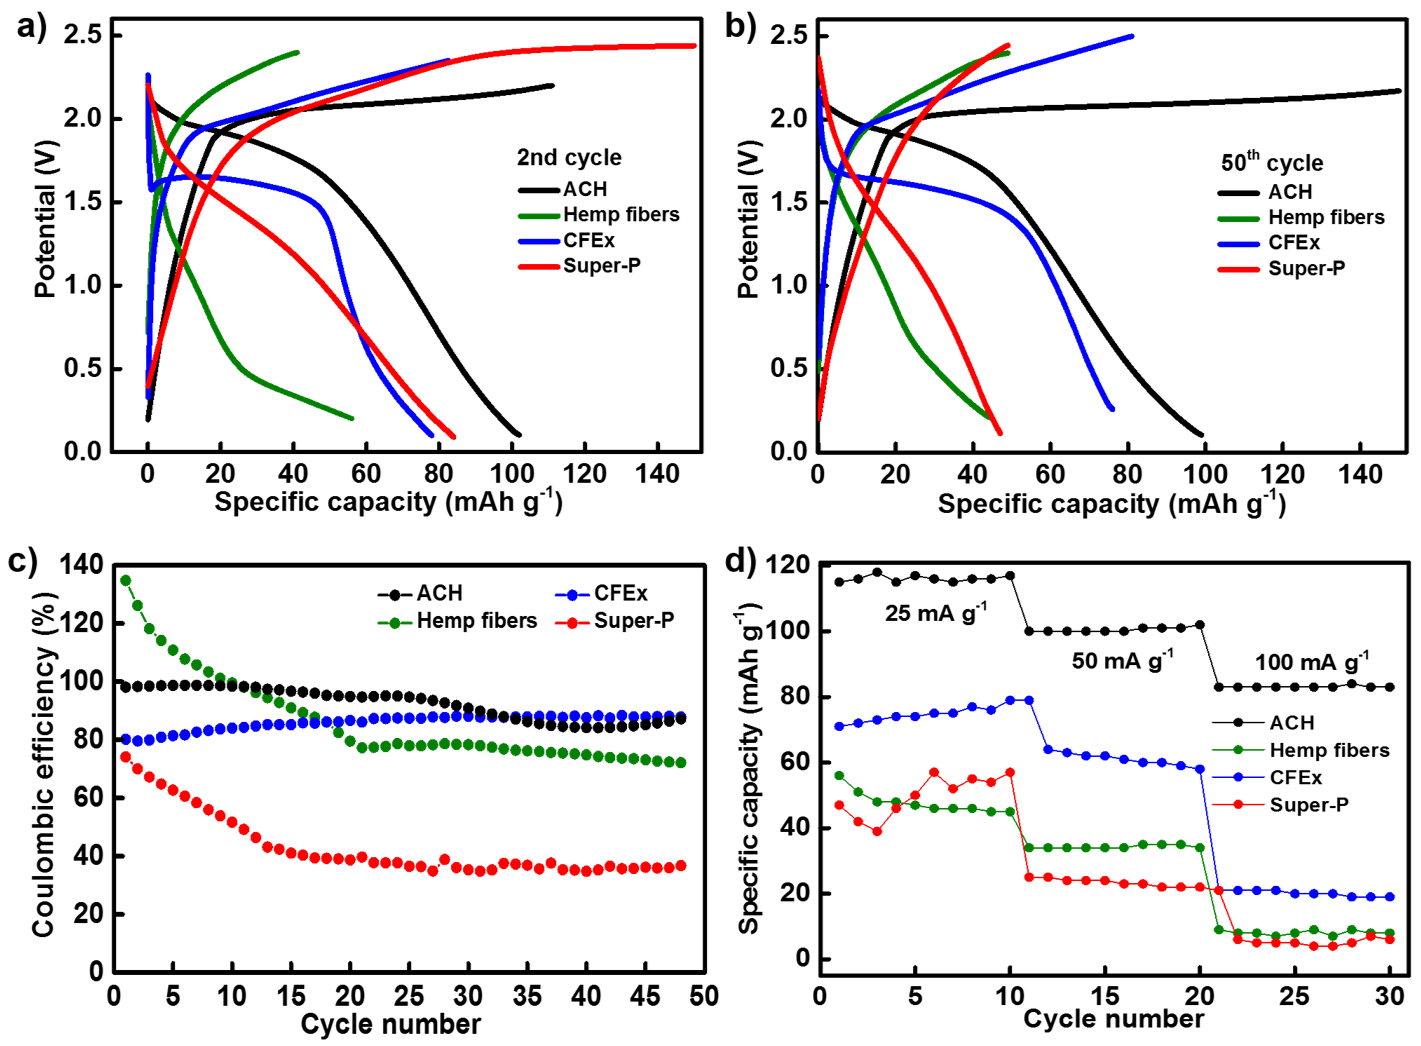
\includegraphics[width=\textwidth]{Figures/chap5fig/cdcall}
    \caption{Specific capacities of AC (human hair, hemp fibers), CFEx and SPCB in their a) first and b) 50$^{th}$ cycle at a current rate of 50 mA g$^{-1}$. c) Coulombic efficiencies of cells at a current rate of 50 mAg$^{-1}$. d) Galvanostatic charge/discharge profile of all cells at various current rates ranging from 25 mAg$^{-1}$ to 100 mAg$^{-1}$ in a two-electrode setup against Al$^{3+}$/Al.}
  \label{Figures/chap5fig:cdcall}
\end{figure}

AC derived from human hair and hemp fibers, and SPCB have a non-crystalline structure, however their Raman spectra revealed the presence of a few graphitic planes. Graphitic layers would allow \ce{AlCl4-} ions to intercalate during charging. CFEx (a mixture of \ce{C60} and \ce{C70} fullerenes) does not have a layered structure. Both fullerenes have a cage-like morphology and the chloroaluminates are not small enough to move in and out of them during charge/discharge. We suggest that \ce{AlCl4-} anions migrated through the gaps present in between the fullerenes without altering its molecular structure. Using a \textit{Neware BTS 3000} battery analyser, specific capacities of the cathodes were recorded at a constant current density of 50 mA g$^{-1}$ (cf.\ Figure \ref{Figures/chap5fig:cdcall}a and b). Morphology of the cathodes before and after the cycles were studied using Raman spectroscopy, X-ray diffraction (XRD) patterns and scanning electron microscopy (SEM).

Figure \ref{Figures/chap5fig:cdcall}a and b compares the specific capacities of all cells for their first and 50$^{th}$ cycles. Human hair cathodes exhibited a high capacity of $\sim$100 mAh g$^{-1}$ with coulombic efficiency of $\sim$95$\%$. High surface area due to its porous structure might have led to an additional 'capacitor-like' charge storage \cite{frackowiak_carbon_2001}. Hemp batteries displayed a capacity of 56 mAh g$^{-1}$ in their first cycle, which decreased to 45 mAh g$^{-1}$ after 50 cycles. CFEx displayed a capacity of around 80 mAh g$^{-1}$ with coulombic efficiency of $\sim$90\%. With an initial value of 84 mAh g$^{-1}$, specific capacity of SPCB decreased to 47 mAh g$^{-1}$ with a low coulombic efficiency of $\sim$40\%. Capacity for SPCB and hemp cells decreased considerably after repeated charge/discharge cycles. A low coulombic efficiency (observed in both hemp and SPCB) can be attributed to side reactions in a battery. These may include electrode or electrolyte interactions with impurities, or degradation of the cathode structure (pulverisation) \cite{gyenes_understanding_2015-1}. However, capacity fade for CFEx and human hair cells was minimal. This suggests that CFEx and human hair have a more stable structure and have the potential to store charge reversibly \cite{pramanick_human_2016}.\\


\fbox{\begin{minipage}{35.5em}
\section*{Activation of carbon}
The production of activated carbon consists of carbonisation of a precursor at a temperature below 900$^{\circ}$ C in an inert atmosphere and chemical or physical activation of the carbonised precursor. Activating agents play an important role in determining the porosity of an AC \cite{arenas_effect_2004}. Using alkali hydroxides at high temperature creates micropores which increases the surface area of the material \cite{dong_commercial_2019, liu_hair-based_2017}. In this work, sodium hydroxide (NaOH) was used as the activating agent. The reaction that takes place inside the carbon matrix after adding NaOH is as follows:

\begin{center}
    4NaOH + C $\longrightarrow$ 4Na + 4\ce{CO2} + 2\ce{H2O} \cite{satish_macroporous_2015}
\end{center}

In this reaction, NaOH was reduced to free metal, Na. These atoms in turn expanded the carbon matrix after intercalating into the carbon structure. Increased temperature (750$^{\circ}$ C) forced the  atoms out of the carbon matrix, thus creating micropores. Oxidation of carbon from oxygen atoms of the hydroxide group formed carbon dioxide (\ce{CO2}), providing routes for channeling the sodium atoms into the internal structure, resulting in a well-connected porous structure \cite{satish_macroporous_2015}. The calcinating temperature used here was 750$^{\circ}$ C. Figure \ref{Figures/chap5fig:achsyn} displays a flowchart describing an AC synthesis. \\
\end{minipage}}



\begin{figure}[ht!]
\centering
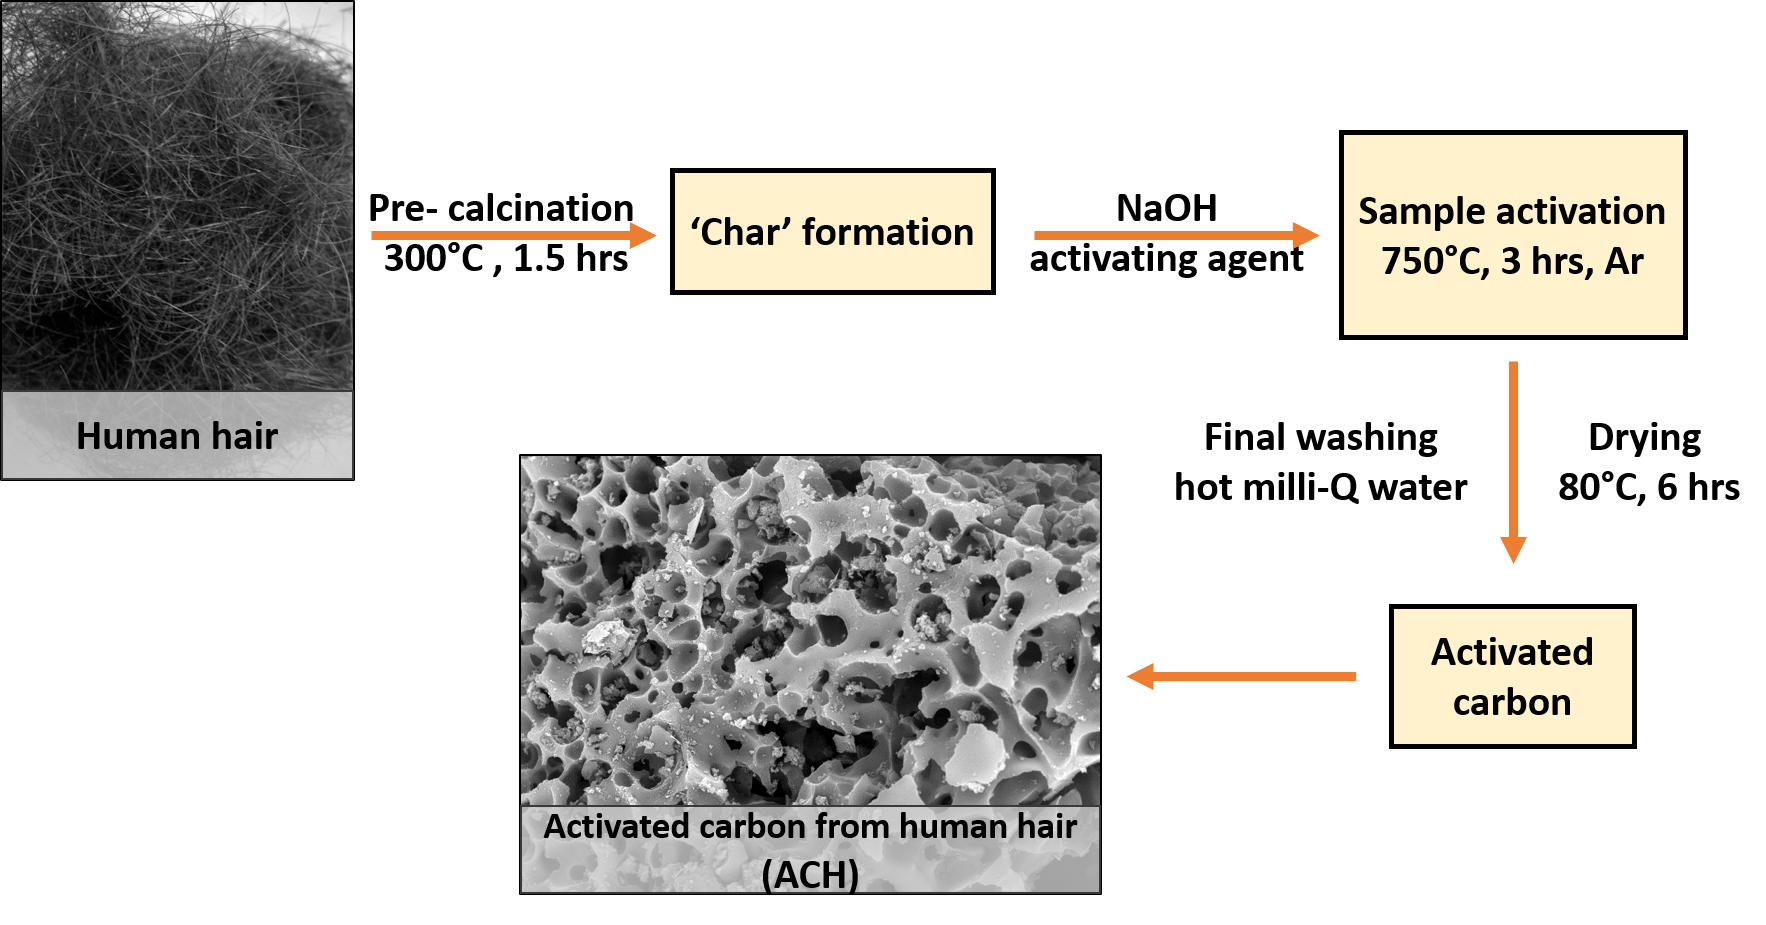
\includegraphics[width=\textwidth]{Figures/chap5fig/achsyn}
\caption{Synthesis of activated carbon (AC) from human hair using NaOH as the activating agent.}
\label{Figures/chap5fig:achsyn}
\end{figure}

\begin{figure}[h!]
\centering
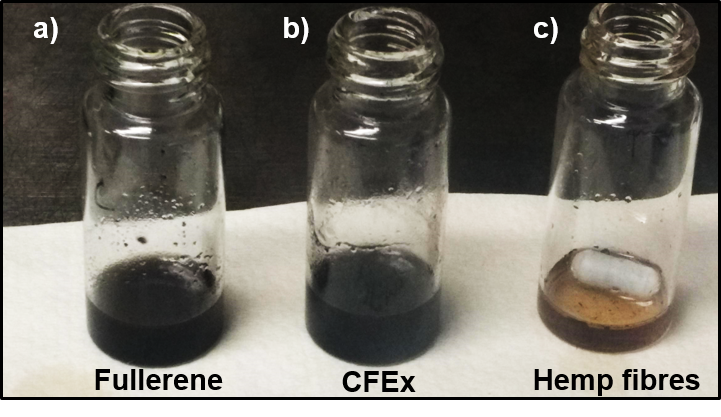
\includegraphics[width=0.75\textwidth]{Figures/chap5fig/cfexsol}
\caption{Comparison of solubility of a) pure \ce{C60} fullerene b) fullerene extract (CFEx) and AC derived from hemp fibers in \ce{AlCl3}/EMImCl ionic liquid electrolyte.}
\label{Figures/chap5fig:cfexsol}
\end{figure}

Fullerenes have a fused-ring structure with a nucleus-to-nucleus diameter of 7.1\AA\ and a van der Waals (vdW) diameter of 11\AA\ in a single crystal. However, they are zero-dimensional materials, which means they cannot provide an efficient path for electron transport or a long-range conductivity \cite{loutfy_fullerene_2002, winkler_two-component_2007}. They are known to be weak battery materials owing to their solubility in electrolytes, especially in LIBs \cite{seger_prospects_1991}. To test their solubility in \ce{AlCl3}-EMImCl, 100 mg of CFEx was mixed in the electrolyte and stirred for 24 hours. The solution was left to stand for another 24 hours inside a \ce{N2}-filled glove box. CFEx seemed to dissolve in the RTIL (Figure \ref{Figures/chap5fig:cfexsol}) since no phase separation was observed. It has been reported that poly-sulphides (formed during charge/discharge cycles) are soluble in the electrolyte of a Li-S battery. They form an insulating layer of \ce{Li2S} on the anode, which results in capacity fading \cite{sun_effect_2017}. Since no such effect was observed in aluminium-fullerene cells, the solubility of fullerenes does not seem to impact the charge-storing capacity of CFEx. On the contrary, aluminium-fullerene batteries demonstrated excellent capacity retention at various current rates(Figure \ref{Figures/chap5fig:cdcall}d).   

 \begin{figure}[tbh!]
  \centering
  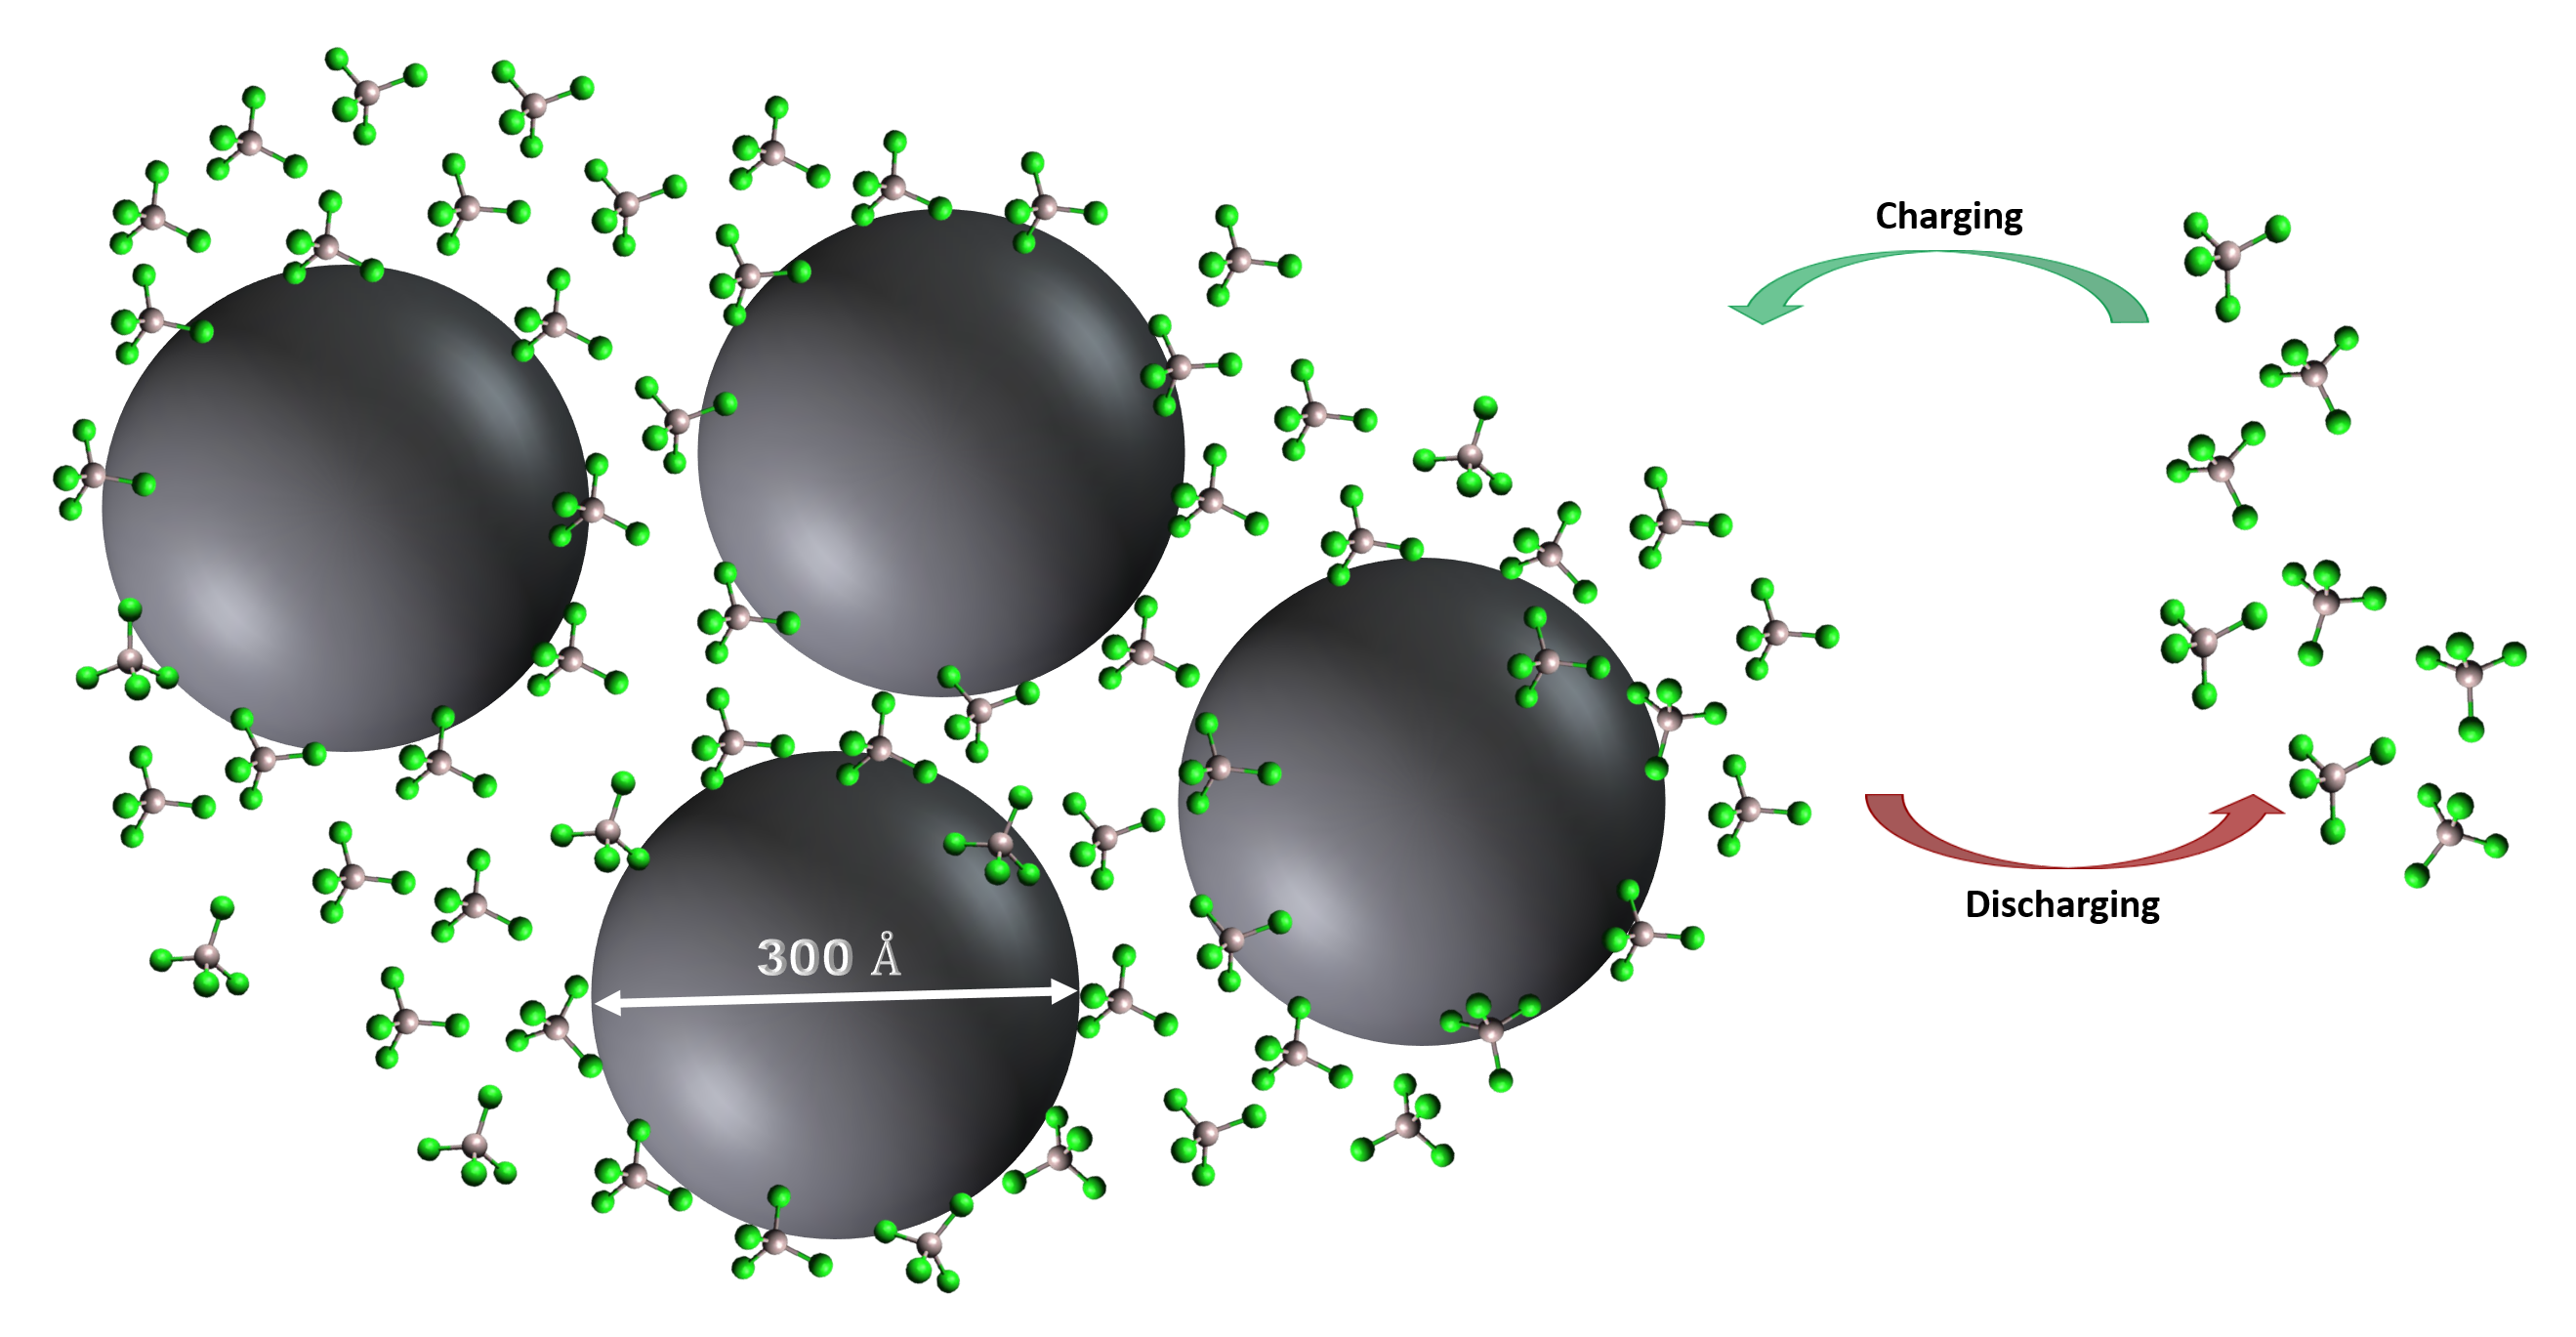
\includegraphics[width=\textwidth]{Figures/chap5fig/superpmech}
    \caption{Suggested mechanism for an aluminium-SPCB cell. \ce{AlCl4-} anions intercalate into the very few graphitic planes in Super-P, while few anions adsorb onto its surface. However, further cycling leads to cathode pulverisation, which results in capacity fading.}
  \label{Figures/chap5figs:superPmech}
\end{figure}

Super-P is an amorphous form of carbon with a high surface area of 62 m$^2$ g$^{-1}$ and a highly disordered structure. The pore sizes range from $\sim$30-50 nm \cite{younesi_analysis_2015}. As a cathode material, SPCB underwent the highest capacity loss within 30 cycles (45\%). It seems continuous cycling destroyed the structural arrangement of the carbon atoms, which resulted in further alleviated capacity and low coulombic efficiencies.

 \begin{figure}[tbh!]
  \centering
  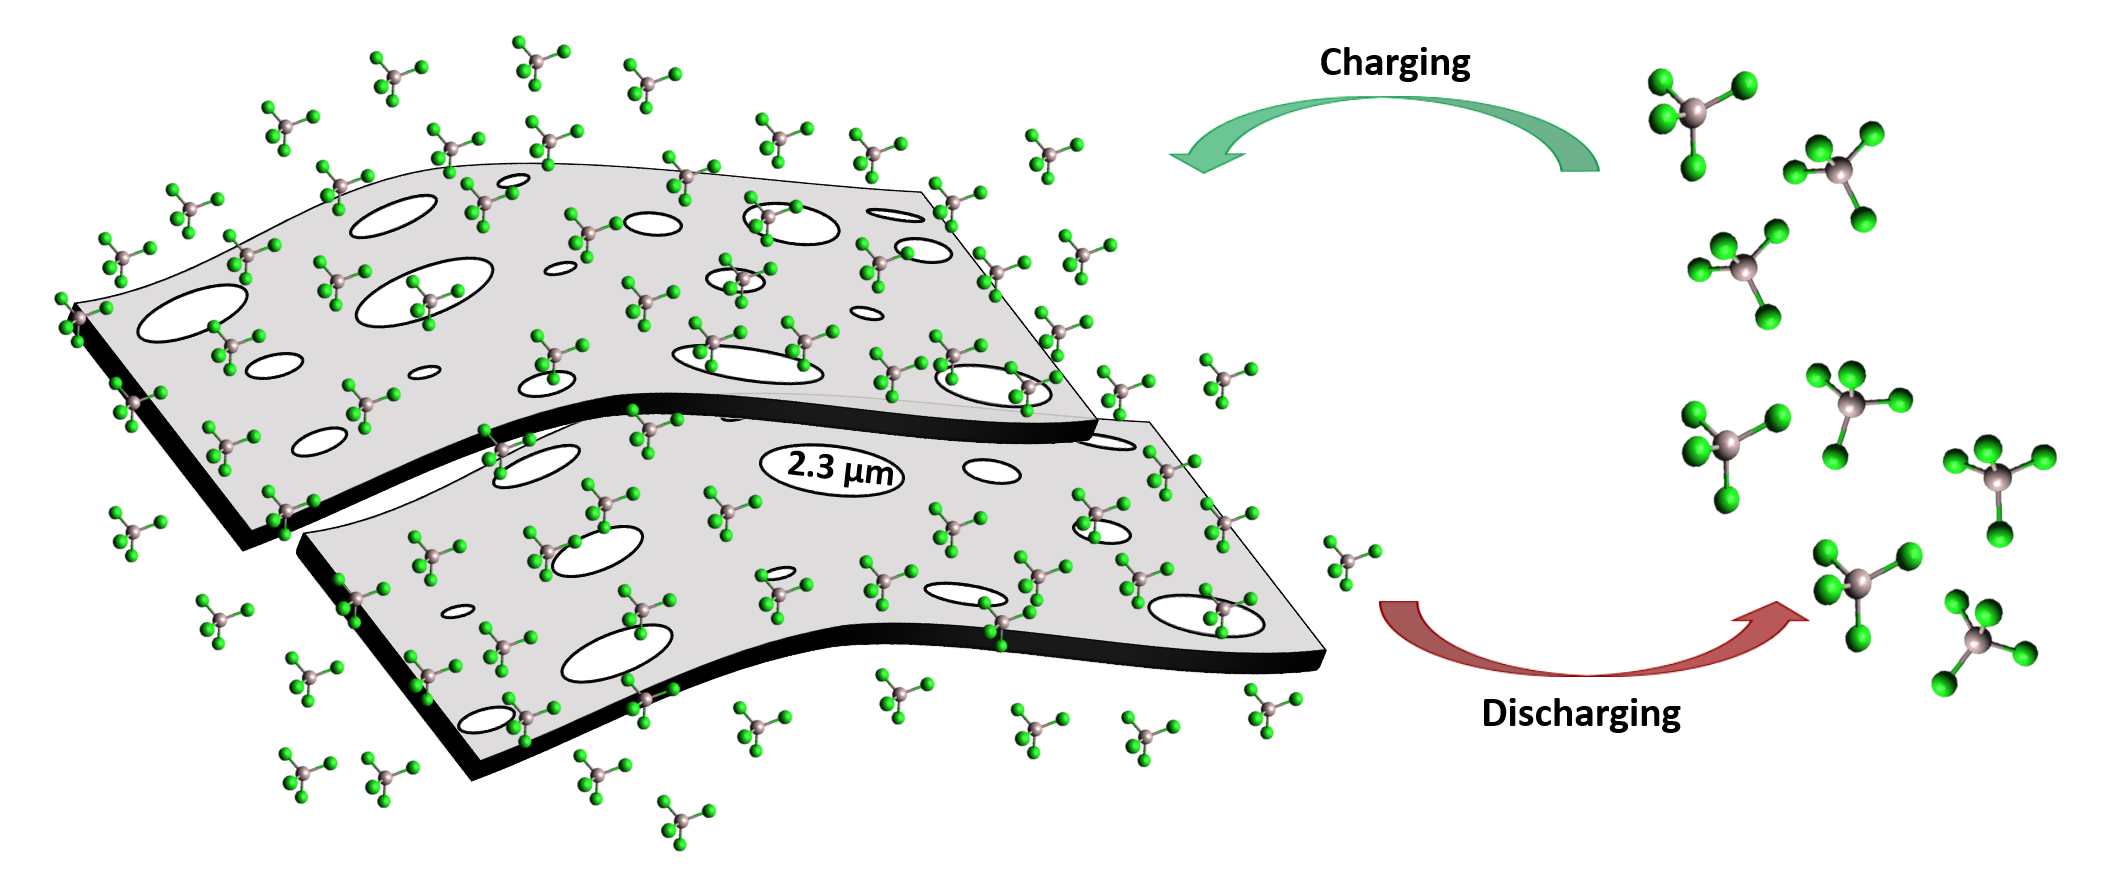
\includegraphics[width=\textwidth]{Figures/chap5fig/hempmech}
    \caption{Suggested mechanism for an aluminum-hemp cell. Hemp fibers have pore sizes which might be as large as 2.0-2.5 $\mu$m allowing the \ce{AlCl4-} to get absorbed on their surface. However, agglomeration of these fibers after a few cycles reduces the number of active sites available for effective charge storage.}
  \label{Figures/chap5fig:hempmech}
\end{figure}

 \begin{figure}[tbh!]
  \centering
  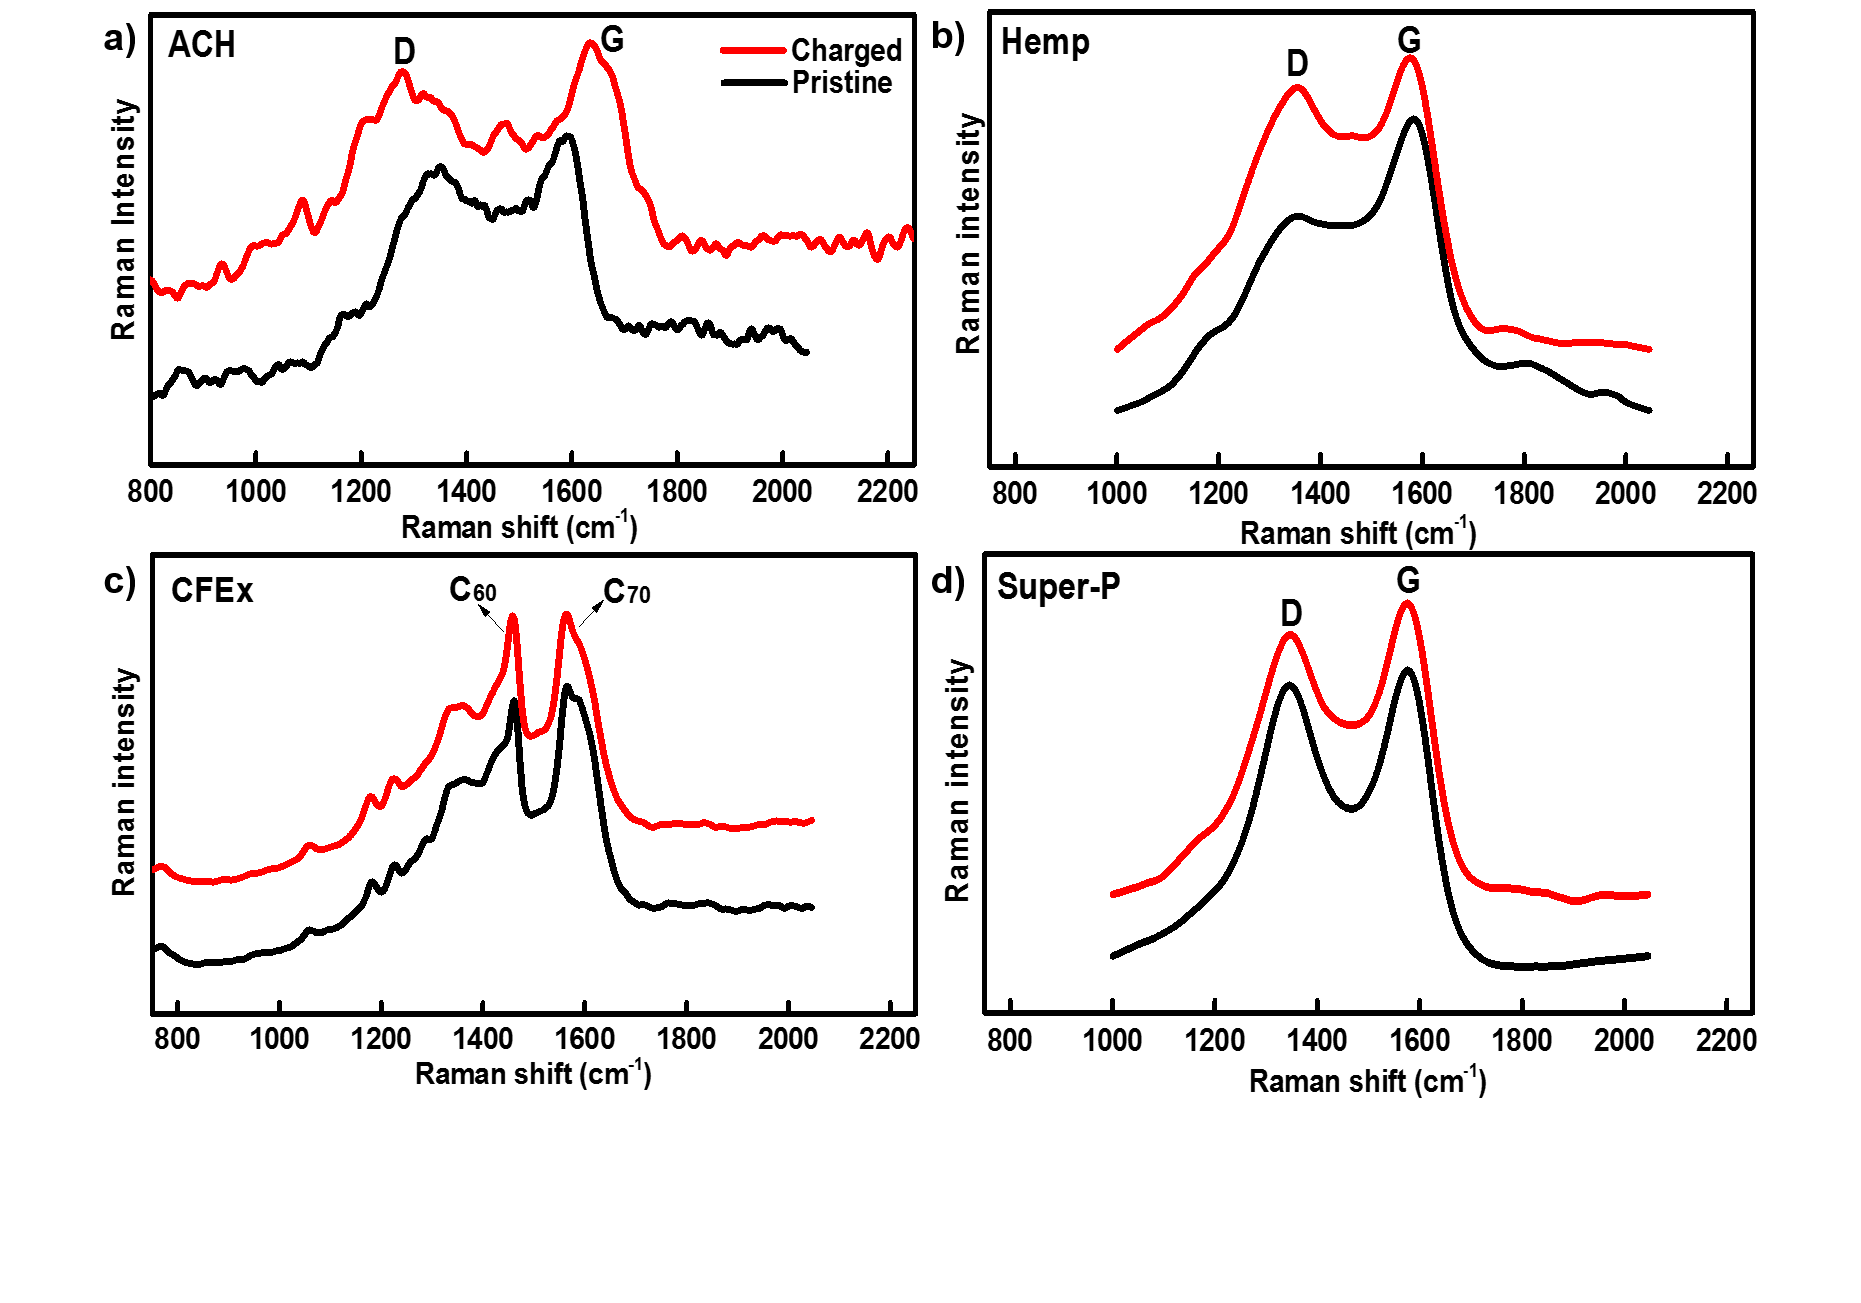
\includegraphics[width=\textwidth]{Figures/chap5fig/Raman}
    \caption{Raman spectra of pristine (in black) and charged (in red) a) CFEx, b) AC from hemp fibers, c) from human hair (ACH) and d) Super-P cathodes displaying presence of both D and G bands.}
  \label{Figures/chap5fig:Raman}
\end{figure}

It has been previously established that chloroaluminates intercalate into the graphitic planes during charging \cite{lin_ultrafast_2015-3}. Since both AC and SPCB cathodes tested in this work have graphitic planes present in them, we compared the pristine and charged electrodes only. Figure \ref{Figures/chap5fig:Raman} displays the Raman spectra of the pristine and charged (intercalated) cathodes. Pristine hair, hemp and SPCB cathodes had a significant D-band present in them, indicating absence of an ordered structure (at $\sim$1300 cm$^{-1}$ for human hair, 1329.7 cm$^{-1}$ for hemp fibers, and 1352.0 cm$^{-1}$ for SPCB). Broad peaks at about 1600 cm$^{-1}$ and about 1350 cm$^{-1}$ arise from \ce{sp2} clusters like $\alpha$-carbons with bond angle disorder \cite{shimodaira_raman_2002}. Raman spectra of CFEx in Figure \ref{Figures/chap5fig:Raman}c displayed the characteristic features of both \ce{C60} and \ce{C70} molecules. A 'pentagonal pinch mode', usually observed in a \ce{C60} Raman spectrum, was present at 1460 cm$^{-1}$. \ce{C70} has multiple bands because it has a reduced molecular symmetry, which increases the number of vibrational modes, consequently increasing the number of active Raman bands \cite{kimbrell_analysis_2014}. It was interesting to note that the spectra of charged CFEx looked strikingly similar to the pristine ones, Figure \ref{Figures/chap5fig:Raman}c. Since Raman spectroscopy is sensitive to minute differences in the molecular morphology, results suggested that the fullerenes did not undergo any significant structural change during cycles. Charged AC (from hair) cathodes showed an increased full-width at half maxima (FWHM), which suggested an increase in the lattice defects and structure deformities. Obviously, these defects arise after intercalation of chloroaluminates into the few graphitic planes present in the carbon matrix. Furthermore, a highly porous structure allows surface adsorption of charge carrying species (much like in super-capacitors) \cite{beguin_carbons_2014}. Intercalation into graphitic planes/micropores, along with surface adsorption of chloroaluminates, result in aluminium-hair batteries performing better than other materials by storing more charge \cite{brezesinski_ordered_2010}. Schematic of an aluminium-hair battery is illustrated in Figure Figure .

 \begin{figure}[h!]
  \centering
  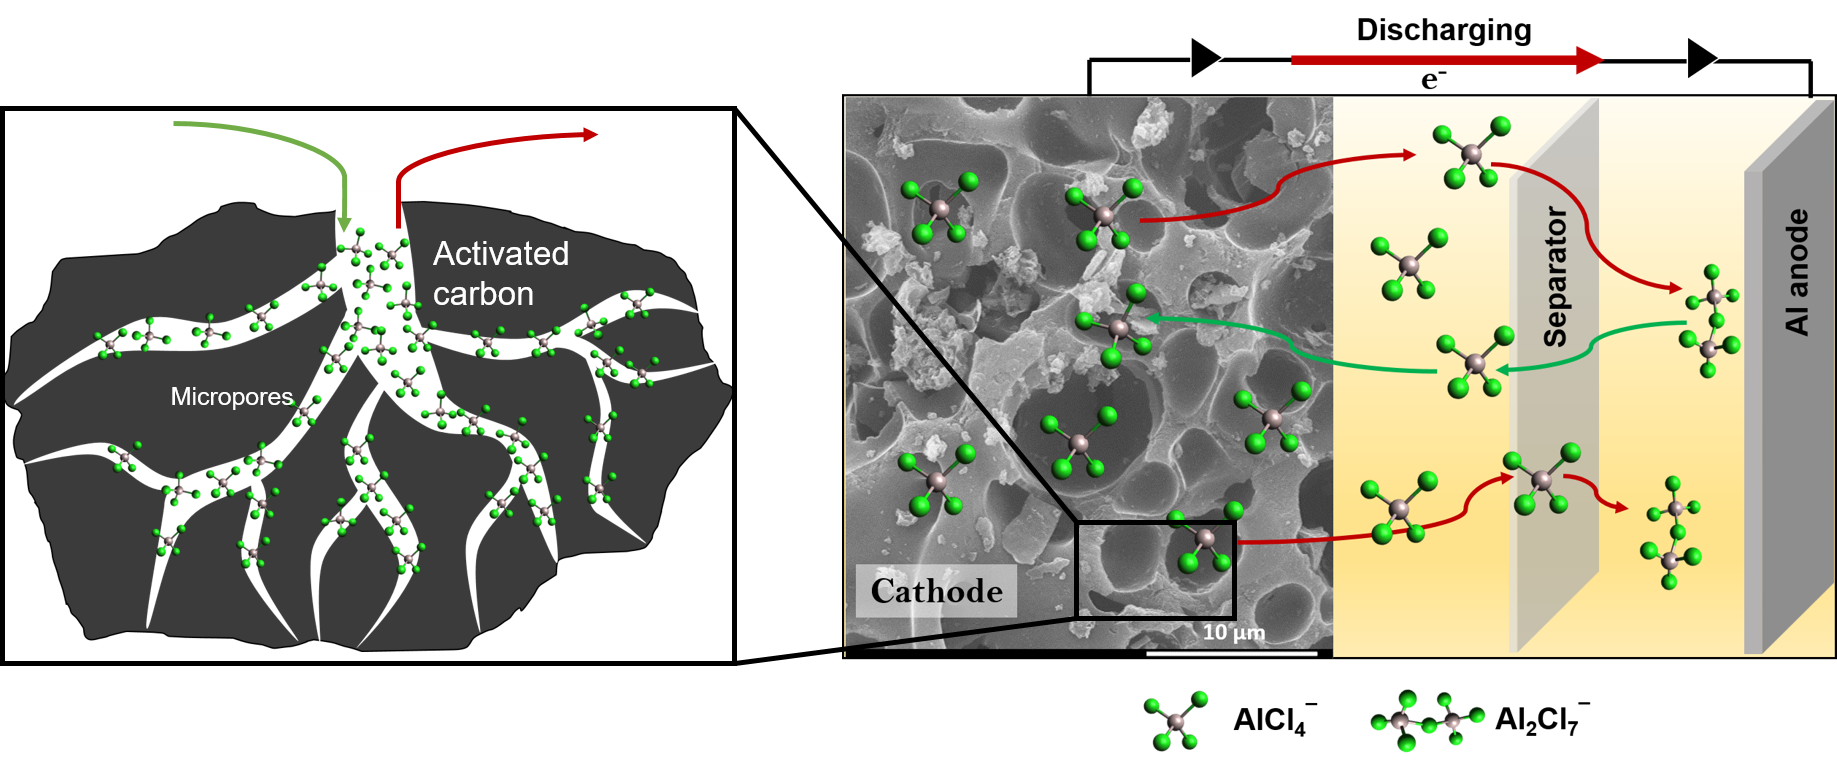
\includegraphics[width=\textwidth]{Figures/chap5fig/achmech}
    \caption{Suggested mechanism for an aluminium-human hair cell. Chloroaluminates (\ce{AlCl4-}) intercalate into the few graphitic planes and micro/mesopores present in them, in addition to surface adsorption of ions displaying both Faradaic and non-Faradaic processes for charge storage.}
  \label{Figures/chap5fig:achmech}
\end{figure}

%contains about 51\% carbon, 17\% nitrogen, 21\% oxygen, 6\% hydrogen, 5\% sulfur, and trace amounts of iron, magnesium, arsenic, chromium and various minerals \cite{lee_chemistry}.  
Hemp fibers and SPCB had a highly disordered structure to begin with. Repeated intercalation or absorption of ions on their surface in the first few cycles would have further increased the lattice defects, which is one of the reasons why hemp and SPCB batteries failed to retain their capacity. However, CFEx does not have graphitic planes to intercalate chloroaluminate ions. Since the fullerenes have a very high surface area, surface adsorption of ions is highly likely \cite{adams_van_1994}. Furthermore, it might be possible for the anions to seep through the gaps present in between two fullerenes (as shown in Figure \ref{Figures/chap5fig:cfexmech}) and for the surface-based redox processes to take place in a systematic way.

 \begin{figure}[tbh!]
  \centering
  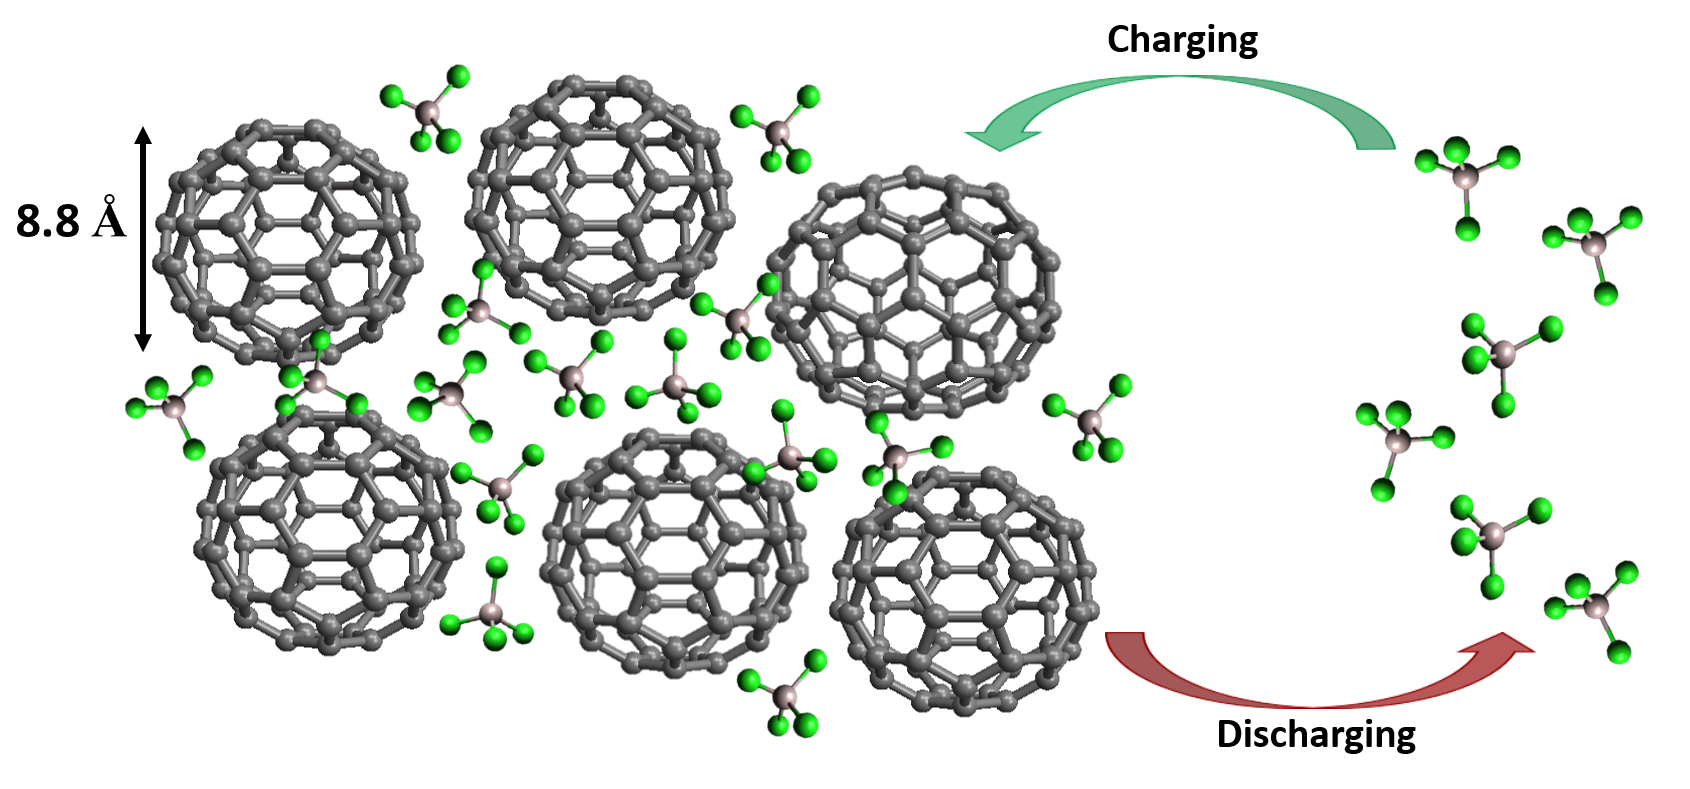
\includegraphics[width=\textwidth]{Figures/chap5fig/cfexmech}
    \caption{Suggested mechanism for a fullerene cell. \ce{AlCl4-} ions seeping in through the gaps present between fullerene molecules.}
  \label{Figures/chap5fig:cfexmech}
\end{figure}

\begin{figure}[tbh!]
  \centering
  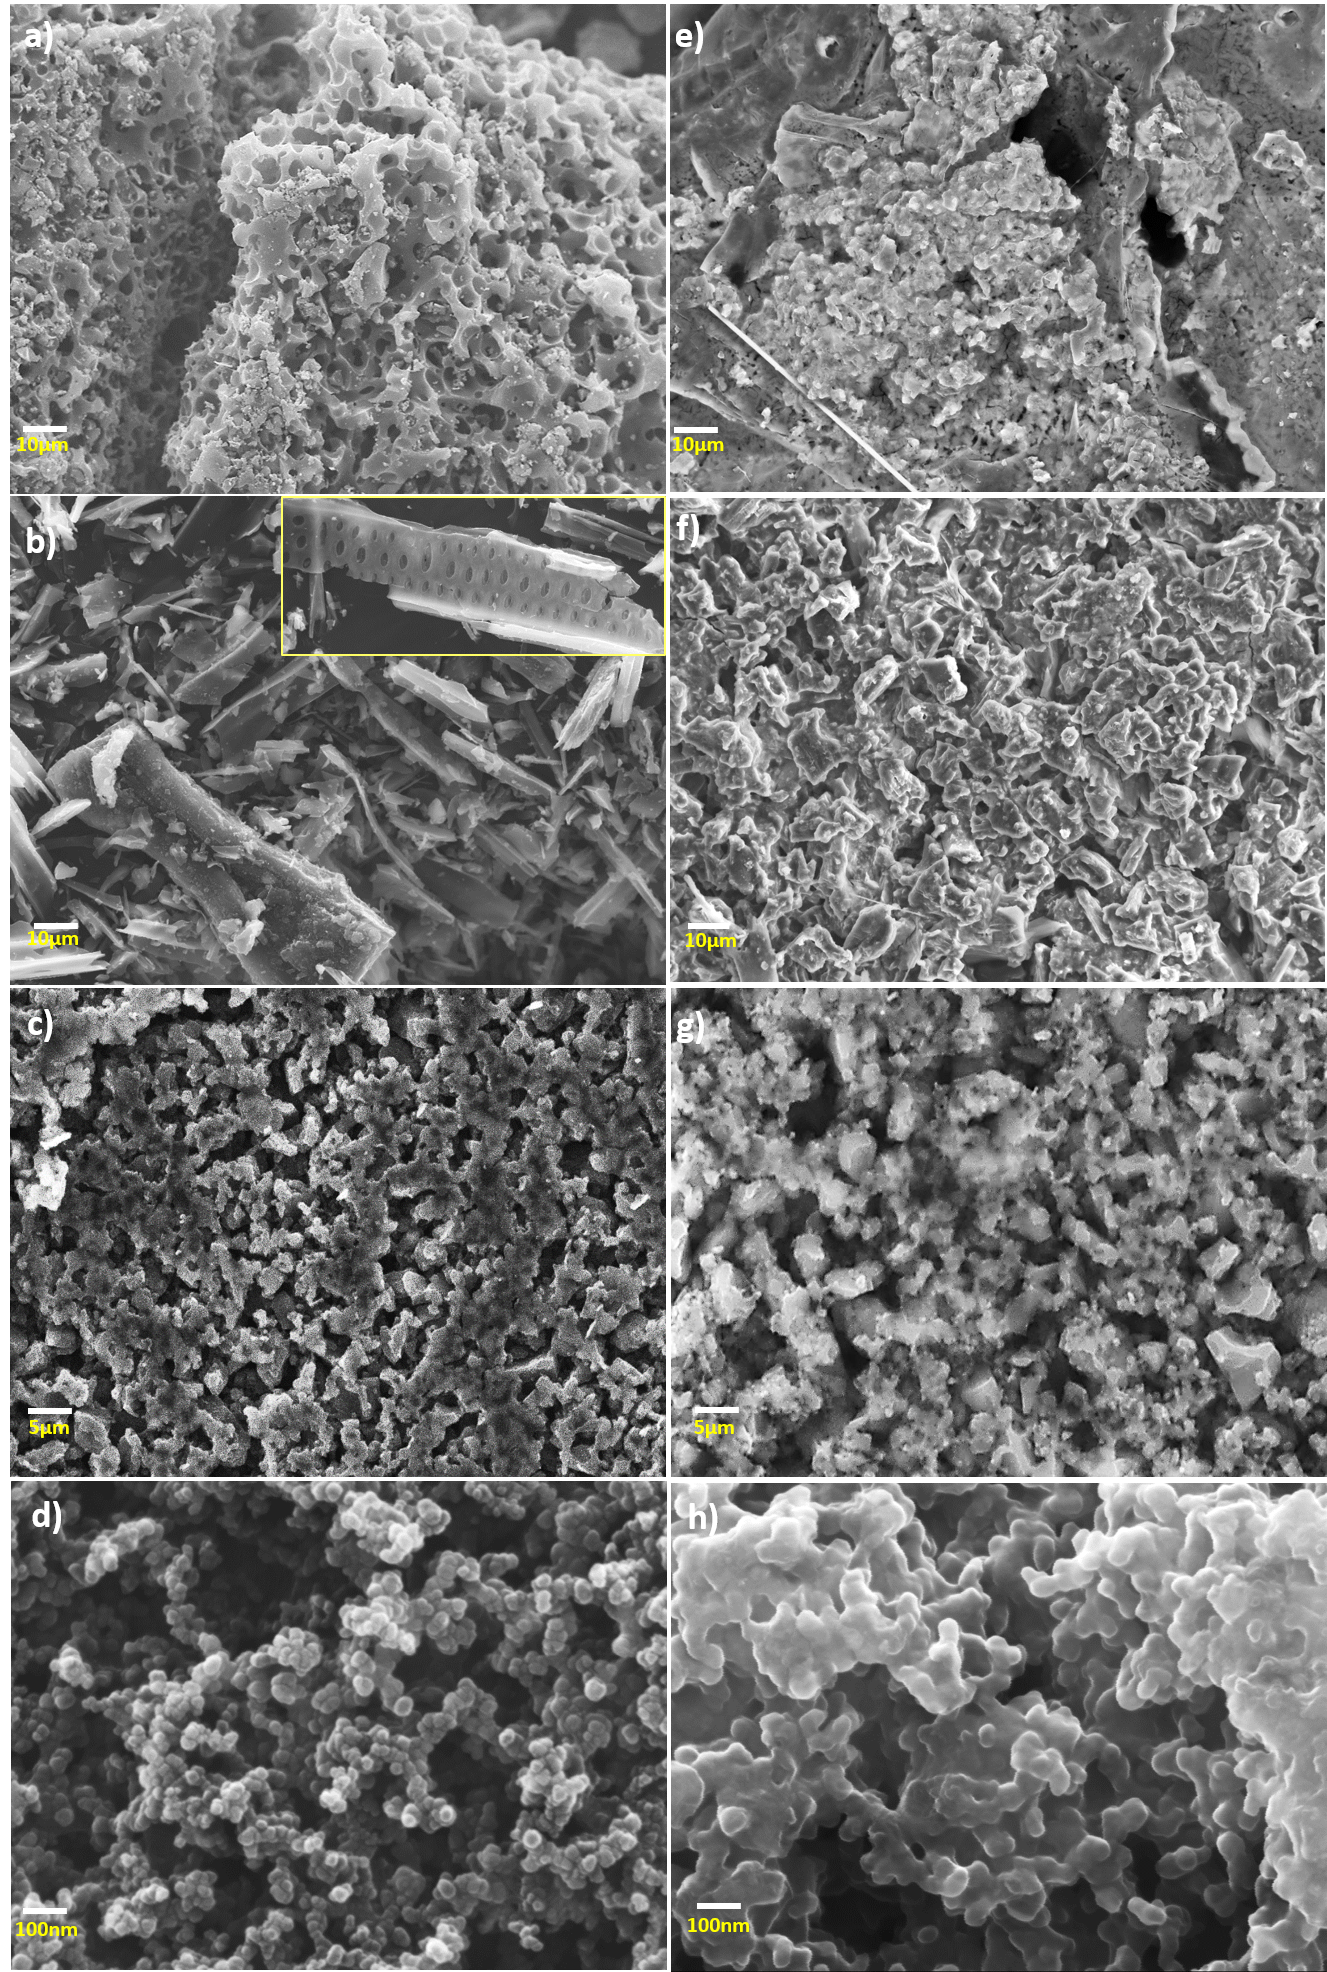
\includegraphics[width=0.6\textwidth]{Figures/chap5fig/SEM}
    \caption{Scanning electron microscopy (SEM) images comparing pristine a) human hair, b) hemp, c) CFEx and d) SPCB and charged e) human hair, f) hemp, g) CFEx and h) SPCB cathodes. Hemp fibers and SPCB undergo permanent changes after charge/discharge cycles and fail to retain capacity.}
  \label{Figures/chap5fig:SEM}
\end{figure}

Figure \ref{Figures/chap5fig:SEM} shows the SEM images of pristine (Figure \ref{Figures/chap5fig:SEM}a, b, c and d) and charged (\ref{Figures/chap5fig:SEM}e,f,g and h) cathodes of all carbon materials. AC has a highly porous structure as seen in Figure \ref{Figures/chap5fig:SEM}b and d). However, hemp cathodes lost their porosity and degraded after 30 cycles, Figure \ref{Figures/chap5fig:SEM}f). Significant agglomeration was observed in SPCB as well (Figure \ref{Figures/chap5fig:SEM}d) and h). It was interesting to note that the cycled AC (from hair) and fullerene cathodes did not undergo any significant changes after cycles. 

\begin{figure}[tbh!]
  \centering
  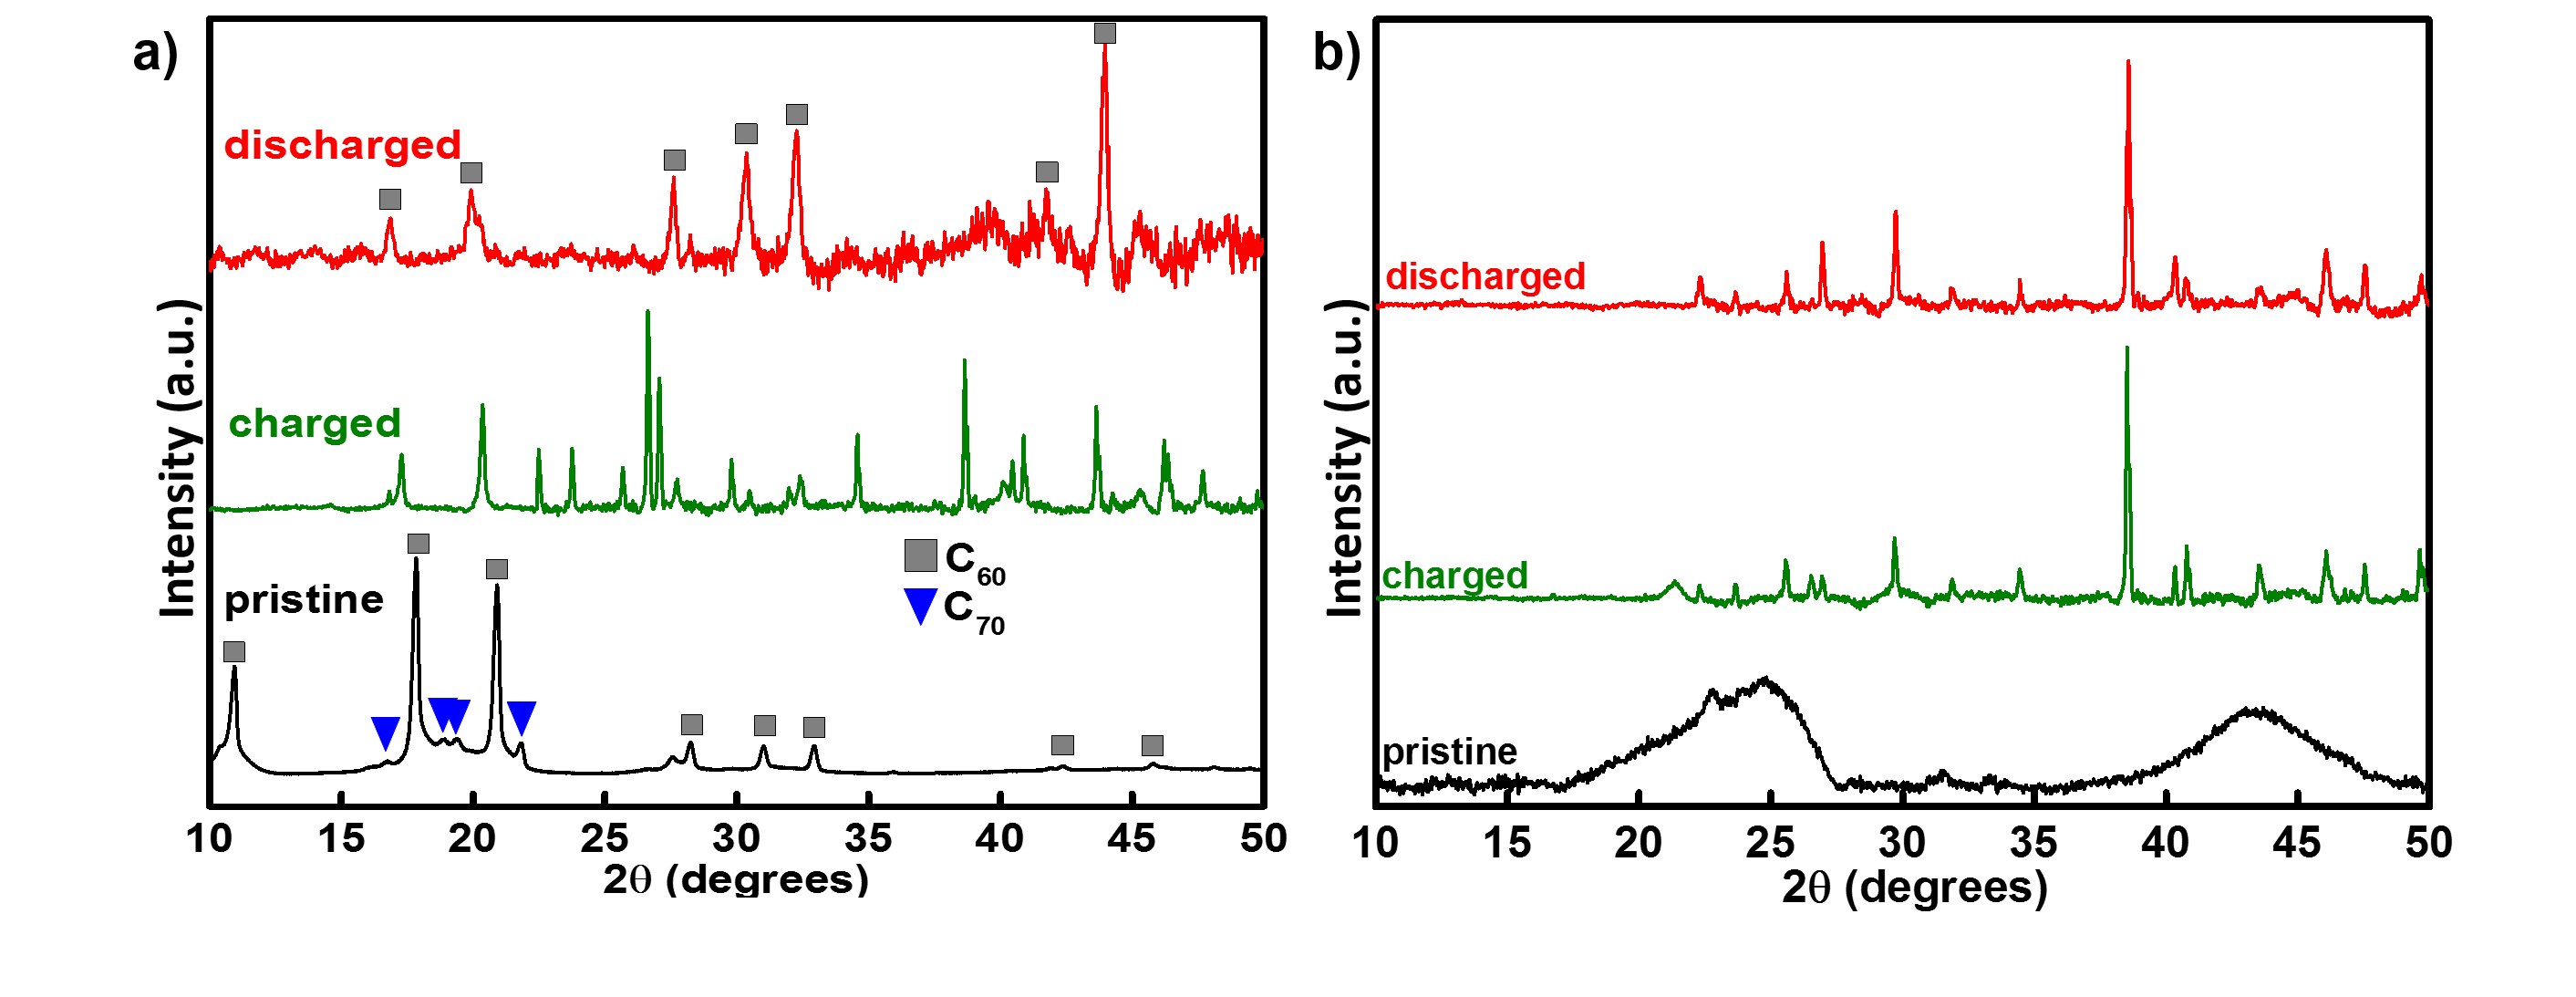
\includegraphics[width=\textwidth]{Figures/chap5fig/XRD}
    \caption{X-ray diffarction patterns of a) CFEx and b)human hair cathodes to study changes in their lattice after galvanostatic cycles in a two-electrode setup against \ce{Al$^{3+}$/Al} with characteristic peaks marked for \ce{C60} (in grey boxes) and \ce{C70} (in blue inverted trainagles).}
  \label{Figures/chap5fig:XRD}
\end{figure}

To further explore the structural stability and the mechanism in CFEx and hair batteries, X-ray diffraction patterns were examined. Pristine (in black), charged (in green) and discharged (in red) cathodes of CFEx and human hair are showed in Figure \ref{Figures/chap5fig:XRD}a and b respectively. Figure \ref{Figures/chap5fig:XRD}a displayed the characteristic peaks of both \ce{C60} and \ce{C70} at 2$\theta$ values of 10.9$^{\circ}$, 17.8$^{\circ}$, 20.9$^{\circ}$ and 28.2$^{\circ}$ for \ce{C60} and 18.9$^{\circ}$, 19.3$^{\circ}$ and 21.8$^{\circ}$ for \ce{C70} molecules. New diffraction peaks at lower 2$\theta$ values appeared for charged electrodes. However, after discharge, the XRD patterns looked similar to the diffraction peaks of the pristine cathode. This data strongly suggests a reversible process taking place during cycles. To confirm, we calculated the unit cell lattice parameters for both pristine and charged cathodes for a \ce{C60} molecule. The unit cell had a tetragonal crystal system with space group of P42/ mmc and a space group number 131 (ICDD: 04-013-1339). Lattice parameters 'a' and 'b' for the charged cathode increased from 9.06 \AA\ to 9.57 \AA\ and 'c' increased from 15.03 \AA\ to 15.65 \AA, as shown in Figure \ref{Figures/chap5fig:cfexcrys}a and b. Lattice parameters of a discharged fullerene were closer to pristine values. These changes suggested a reversible insertion of chloroaluminates into the free spaces between fullerene molecules taking place. A possible site for \ce{AlCl4-} intercalation is depicted in Figure \ref{Figures/chap5fig:cfexcrys}c. XRD patterns of human hair cathodes were inconclusive (Figure \ref{Figures/chap5fig:XRD}b). Pristine cathode showed broad peaks that demonstrate an amorphous and highly porous structure. However, the material became more symmetrical and crystalline after cycles. Charged and discharged cathodes exhibited similar looking patterns implying no change in the newly formed crystal lattice during cycles. It is to be noted that presence of crystallinity in an active material does not limit the surface-based charge storing capacity \cite{kim_synthesis_2006, jow_factors_2018}. 

\begin{figure}[tbh!]
  \centering
  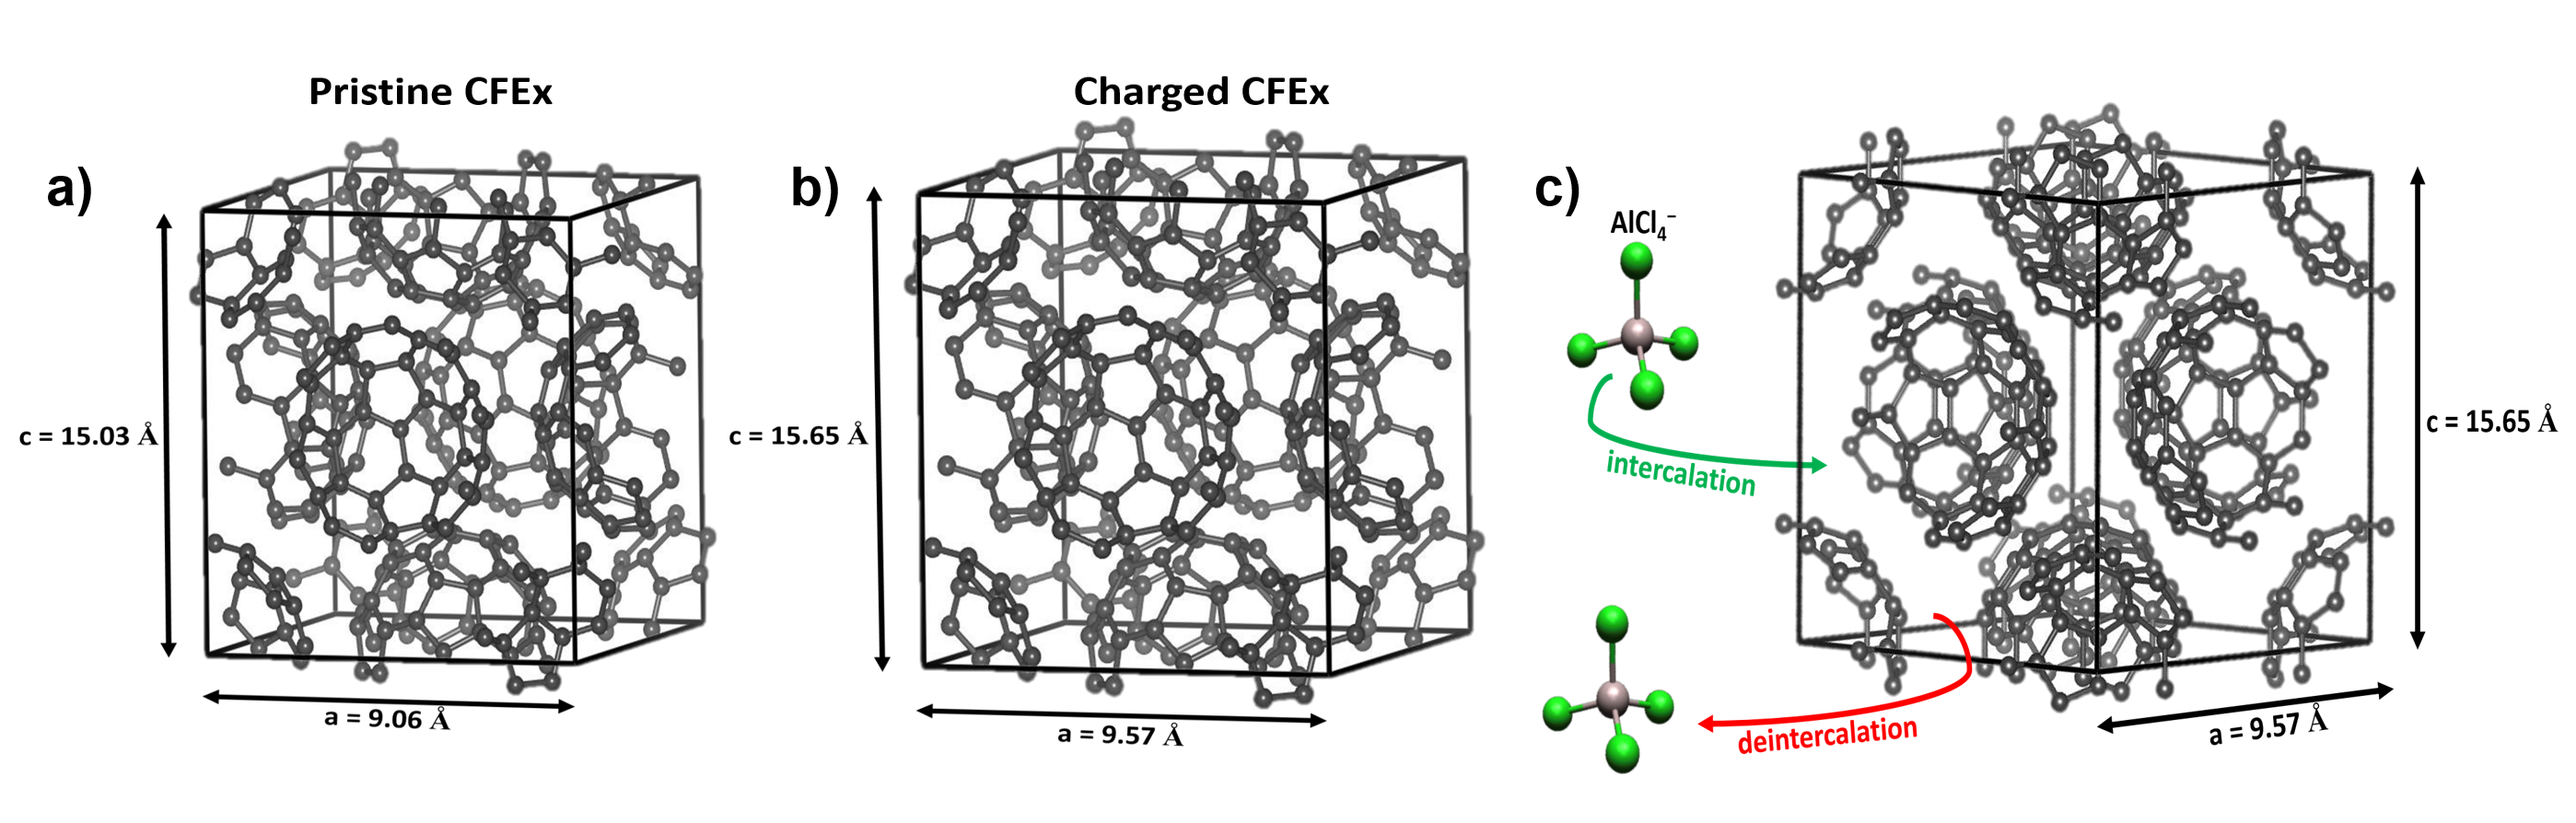
\includegraphics[width=\textwidth]{Figures/chap5fig/cfexcrys}
    \caption{Changes in the lattice parameters of a \ce{C60} unit cell. a) Pristine \ce{C60}unit cell, b) charged \ce{C60}unit cell with increased parameters suggesting a uniform shift in the lattice after charge/discharge. c) Expected intercalation sites of \ce{AlCl4-} ions in the unit cell.}
  \label{Figures/chap5fig:cfexcrys}
\end{figure}

%Charged Super-P and hemp fiber electrodes underwent degradation and appeared clumped together resulting in capacity decay. This was visible from their electrochemical results where a rapid decrease in capacity and cell efficiency was noted. 
%XPS analysis results... C 1s 
\begin{figure}[tbh!]
  \centering
  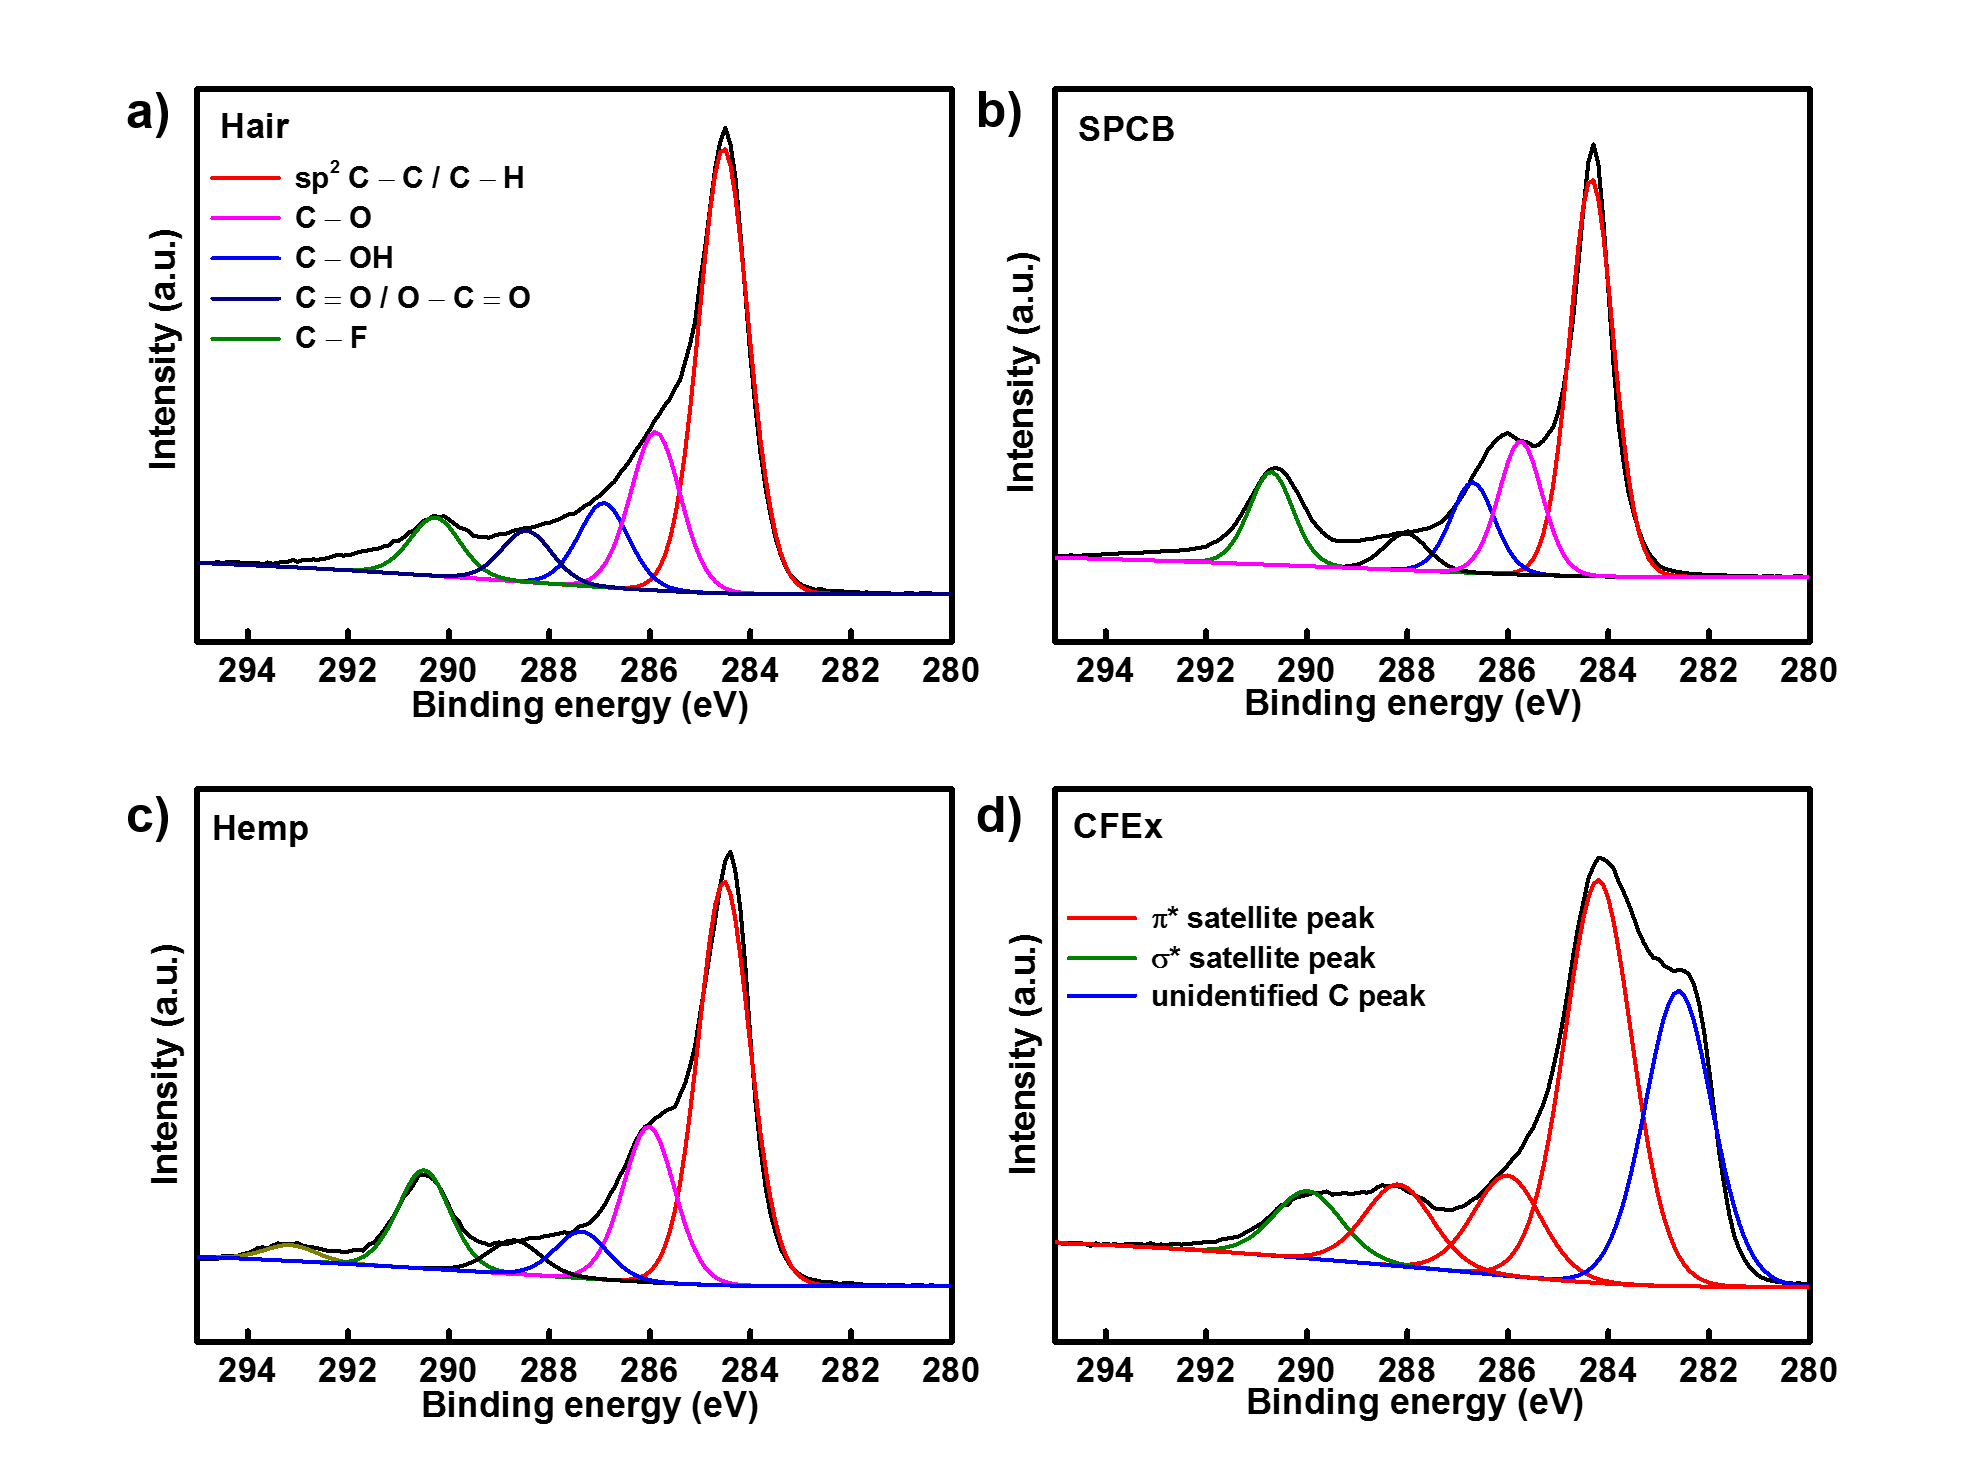
\includegraphics[width=\textwidth]{Figures/chap5fig/XPSC}
    \caption{Carbon 1s XPS spectra of pristine a) hair, b) Super-P, c) hemp fibers and d) CFEx cathodes. While AC from human hair (ACH), hemp fibers and Super-P contain carbonyl functional groups, CFEx cathodes have symmetrical looking $\pi$* and $\sigma$* satellite peaks.}
  \label{Figures/chap5fig:XPSC}
\end{figure}

XPS spectra of carbon 1s orbital of all pristine cathodes is shown in Figure \ref{Figures/chap5fig:XPSC}. Hair, hemp fibers and SPCB had similar looking peaks for the 1s orbital. All three cathodes displayed peaks for sp$^2$ C-C/ C-H, C-O/ C-OH, O-C=O/ C=O and C-F bonds . Since hair is mainly composed of a protein called keratin (Figure \ref{Figures/chap5fig:keratin}), it can be deduced that multiple chemical environments of carbon, shown in Figure \ref{Figures/chap5fig:XPSC}a), are derived from Keratin. Sulphide bonds are an essential part of this protein and a C-S binding energy is observed at 286.94 eV (blue peak).

\begin{figure}[th!]
\centering
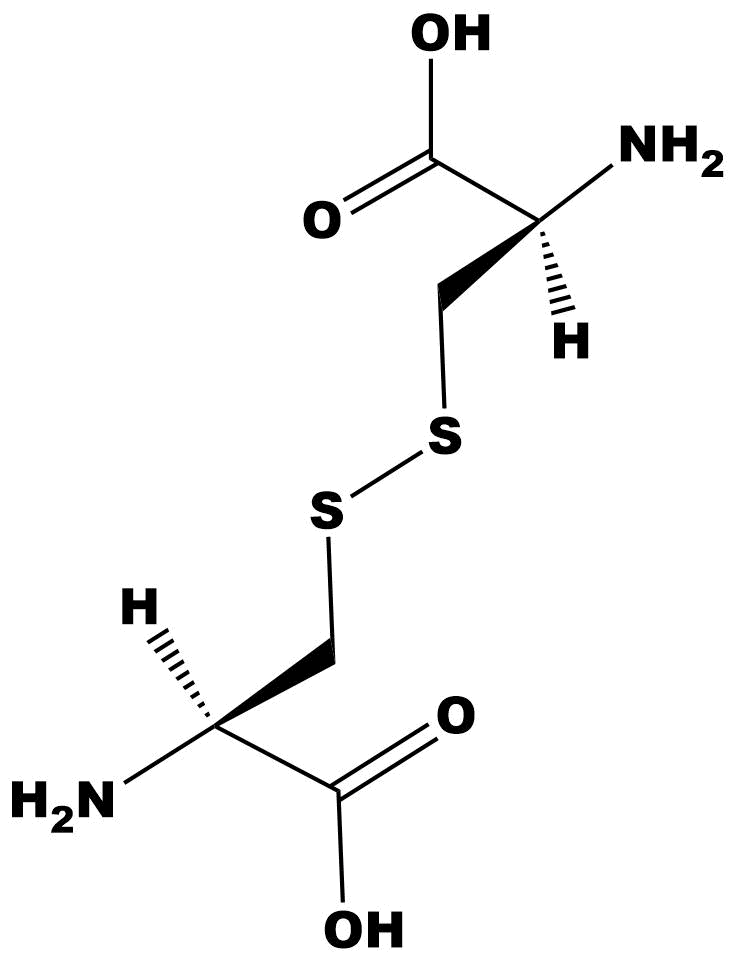
\includegraphics[width=0.5\textwidth]{Figures/chap5fig/keratin}
\caption{Keratin: a protein abundantly found in human hair contains C-O, C=O, C-NH$_2$ bonds.}
\label{Figures/chap5fig:keratin}
\end{figure}

\begin{sidewaystable}
\centering
\caption{Characteristics of commonly used rechargeable batteries.} \label{table2xps}
\begin{tabular}{ |p{2.5cm}|p{2cm}|p{2cm}|p{2cm}|p{1.5cm}|p{2.5cm}|p{2.5cm}|p{2.5cm}|}
\hline
\textbf{Active material} & \textbf{C-H/C-C} & \textbf{C-O/C-OH} & \textbf{C=O/O-C=O} & \textbf{C-F} & \textbf{Pyrrolic N / Pyridinic N} & \textbf{Aliphatic C-O} & \textbf{Aromatic C=O}\\
\hline
Human hair & 284.5 eV & 285.8 eV & 288.4 eV & 290.2 eV & 400.2 eV / 398.3 eV & 533.0 eV & 531.2 eV\\
CFEx & 284.2 eV & 286.0 eV & 288.2 eV & 290.0 eV & 399.3 eV & 531.3 eV & 530.2 eV\\
Hemp fibers & 284.5 eV & 286.0 eV & 288.7 eV & 290.5 eV & 400.3 eV & 532.9 eV & 531.4 eV\\
SPCB & 284.3 eV & 286.7 eV & 288.0 eV & 290.7 eV & 400.2 eV & 532.8 eV & ---\\
\hline
\end{tabular}
\end{sidewaystable}

\newpage

Functional groups that contain oxygen, such as carbonyl and ester groups, improve the wettability of a material, which increases the availability of active surface area \cite{younesi_analysis_2015}. SPCB is produced from partial oxidation of petrochemical precursors \cite{gnanamuthu_electrochemical_2011}. A perfect graphite surface containing only carbon atoms, without heteroatoms like oxygen and sulfur, would give a very well-ordered structure. Presence of impurities such as carbonyl groups creates defects resulting in a less graphitic and more amorphous structure\cite{hao_carbonaceous_2013} and peaks at 288.0 eV in AC and SPCB cathodes confirm that. Spectra for C 1s orbital of CFEx was uniquely different than the others due to presence of several highly symmetrical peaks. The presence of $\pi$ electrons on its surface results in  multiple $\pi$ satellite peaks, which are typical in a \ce{C60} molecule \cite{skryleva_xps_2016}. These peaks appear in both high (in green) and low energy ranges (in red) \cite{erbahar_spectromicroscopy_2016, poirier_carbon_1993}.   

\begin{figure}[h!]
  \centering
  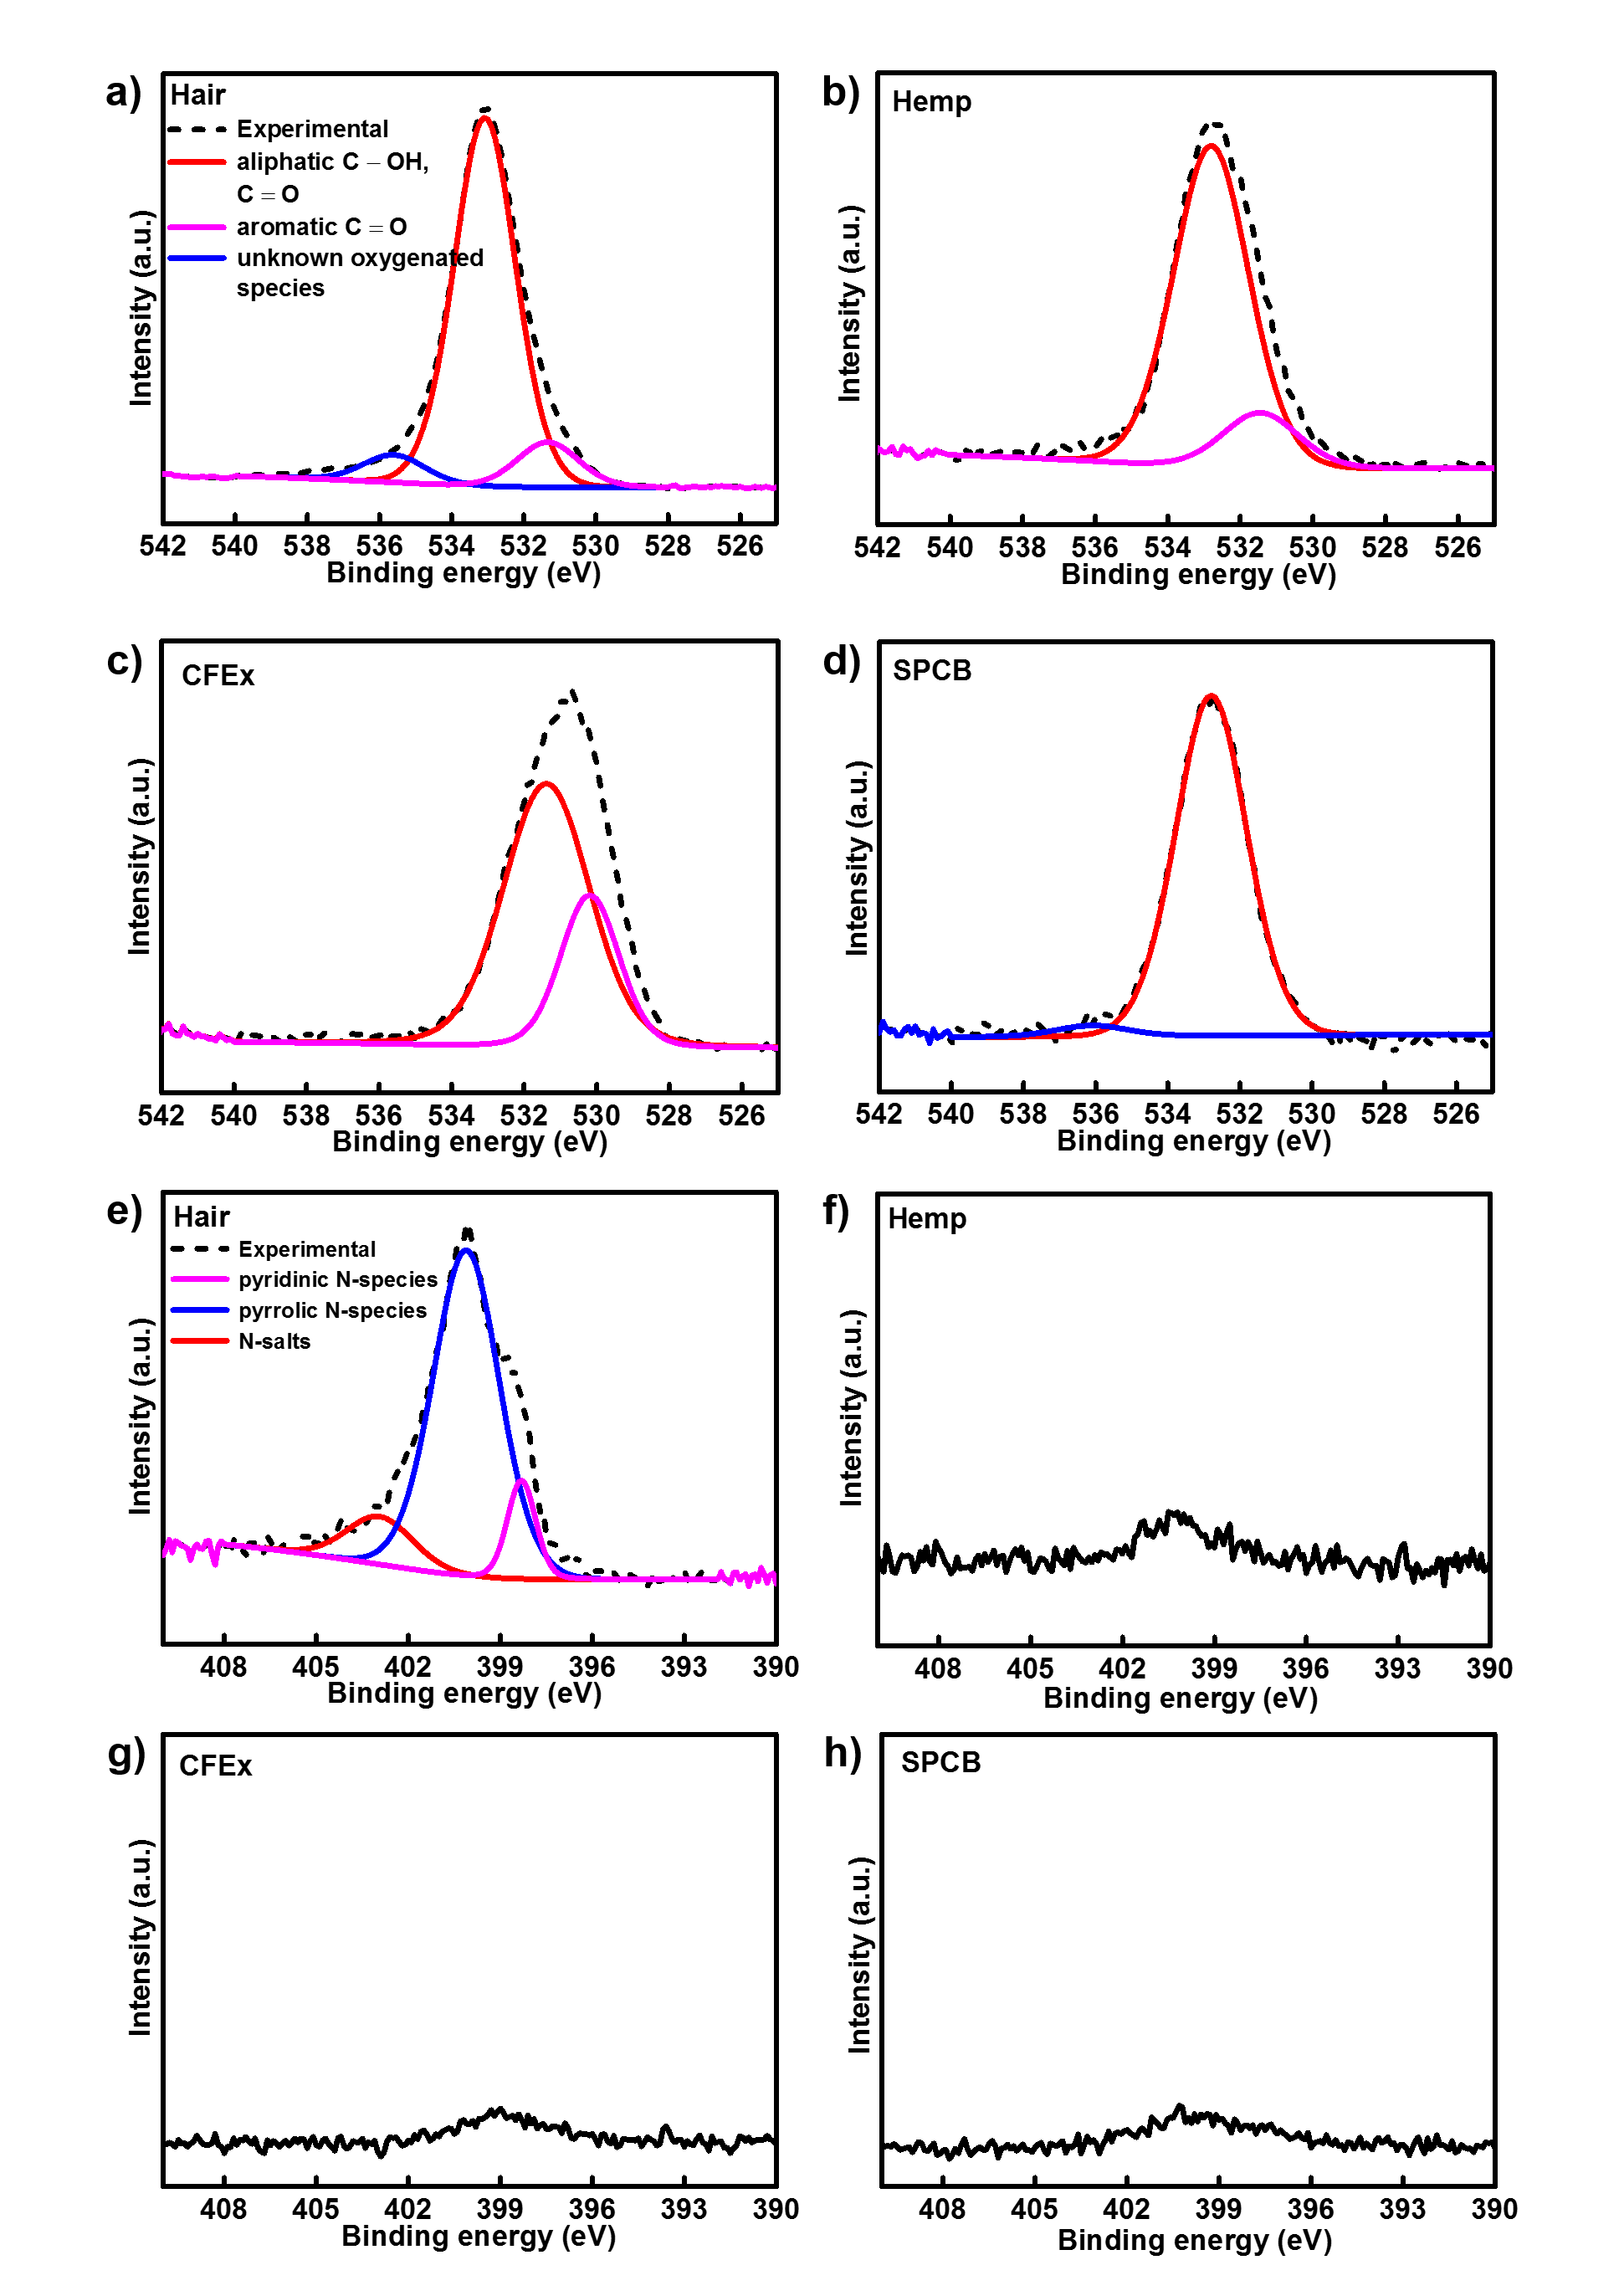
\includegraphics[width=0.8\textwidth]{Figures/chap5fig/XPSON}
    \caption{XPS spectra of O 1s orbital for a) AC from human hair (ACH), b) hemp fibers c) CFEx and d) SPCB cathodes. Hair and hemp fibers contained significant amounts of aliphatic (red) and aromatic (pink) C=O groups  compared to CFEx and SPCB. Binding energies for N 1s orbital of e) hair, f) hemp fibers g) CFEx and h) SPCB cathodes. Human hair displayed distinct binding energies for pyridinic and pyrrolic N-species; hemp fibers, CFEx and SPCB had smaller amounts of surface proteins.}
  \label{Figures/chap5fig:XPSON}
\end{figure}

Figure \ref{Figures/chap5fig:XPSON}a-d shows various binding energies for O 1s orbital. In addition to enhancing the wettability of a material, oxygen containing functional groups make redox reactions feasible \cite{li_effect_2011, oh_oxygen_2014}. Oxygen-containing surface functional groups can provide pseudo-capacitance by reacting with electrolyte ions \cite{bleda-martinez_role_2005}. This might another reason why aluminium-hair batteries performed better than the others. Figure \ref{Figures/chap5fig:XPSoverall} displays the overall spectra of all tested cathodes. Table \ref{table2xps} compiles all the functional groups with their respective binding energies for all tested cathode materials in this work. 

\begin{figure}[th!]
\centering
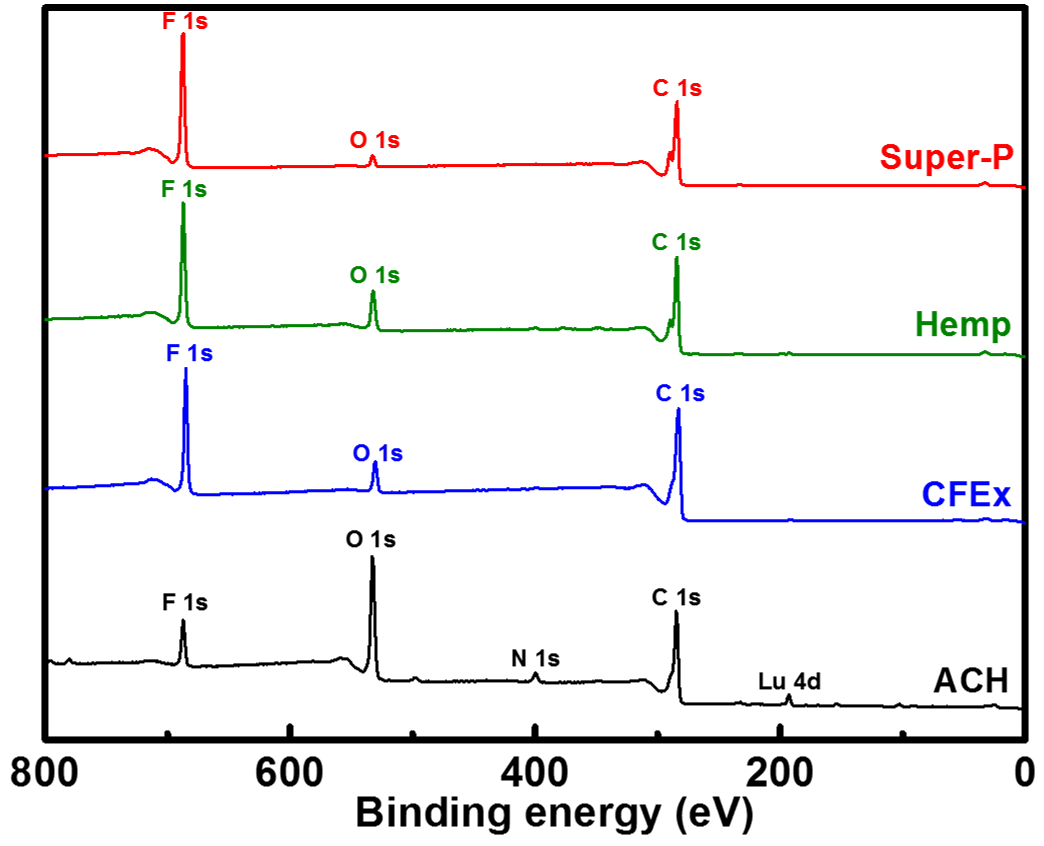
\includegraphics[width=\textwidth]{Figures/chap5fig/XPSoverall}
\caption{Overall spectra of human hair (black), hemp fibers (blue), CFEx (green) and Super-P(red).}
\label{Figures/chap5fig:XPSoverall}
\end{figure}

 \begin{figure}[h!]
  \centering
  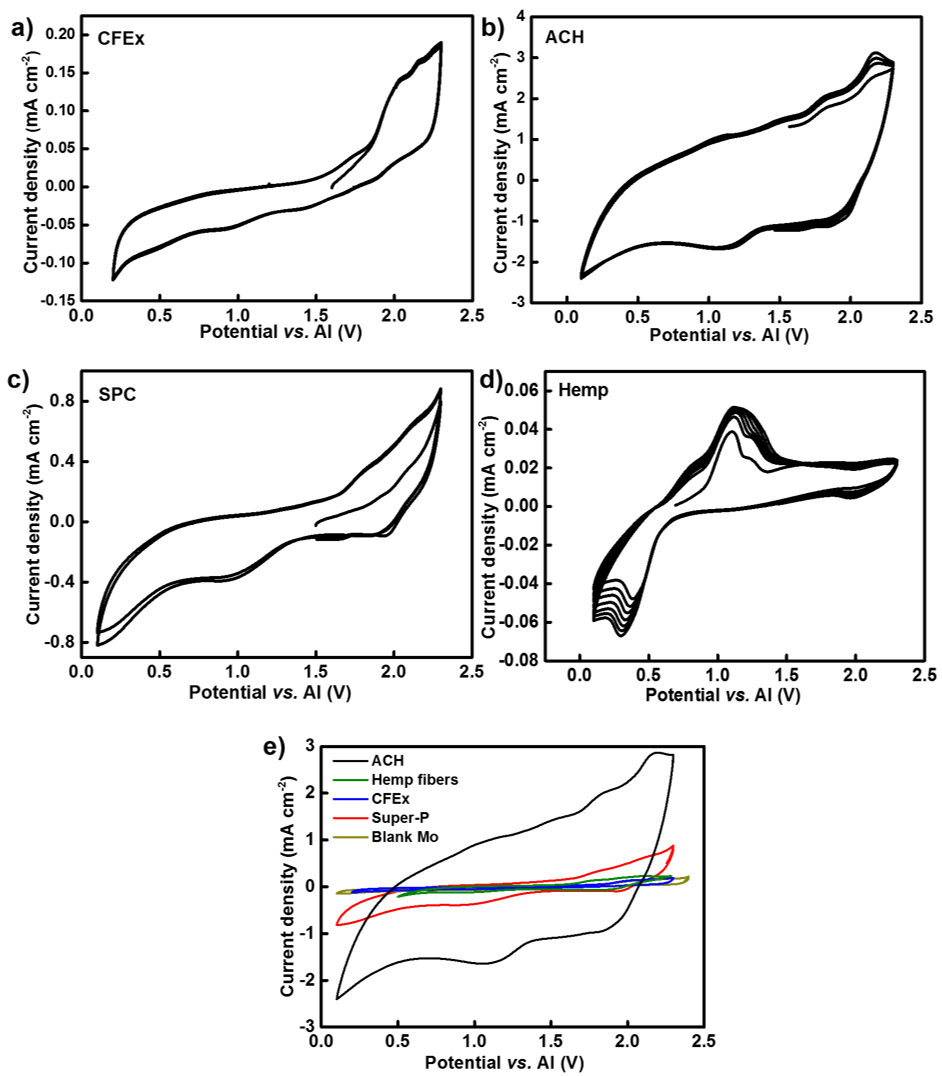
\includegraphics[width=\textwidth]{Figures/chap5fig/CV}
    \caption{Cyclic voltammograms of a) CFEx, b) hair, c) Super-P and d) hemp fibers cathodes at a scan rate of 10 mV s$^{-1}$ against \ce{Al3+}/Al as a counter/reference electrode in a two-electrode setup. ACH cathode observed a larger CV area than other cathodes, which comes from an additional pseudocapacitance, adding capacity to the system.}
  \label{Figures/chap5fig:CV}
\end{figure}

Lastly, to confirm that AC derived from human hair is in fact a psedocapacitive material, we compared cyclic voltammograms of all cathodes at a scan rate of 10 mV s$^{-1}$. Figure \ref{Figures/chap5fig:CV}a-e showed that human hair batteries demonstrated a more rectangular, capacitor-like CV curve. However, redox processes were noticeable at a scan rate of 10 mV s$^{-1}$ and tiny redox peaks were visible (Figure \ref{Figures/chap5fig:CV}b). At a higher scan rate (50 mV s$^{-1}$), the redox peaks disappeared and the material displayed an ideal capacitor-like CV curve, shown in Figure \ref{Figures/chap5fig:hair50mVs} \cite{guan_capacitive_2016, dupont_separating_2015}. 

\begin{figure}[th!]
\centering

\includegraphics[width=\textwidth]{Figures/chap5fig/hair50mVs}
\caption{Cyclic voltammogram of ACH at a scan rate of 50 mV/s in a two electrode setup against \ce{Al3+}/Al showing a capacitor-like behaviour with no visible oxidation-reduction peaks unlike Figure \ref{Figures/chap5fig:CV}b where we distinctly observed redox peaks.}
\label{Figures/chap5fig:hair50mVs}
\end{figure}

\begin{figure}[h!]
  \centering
  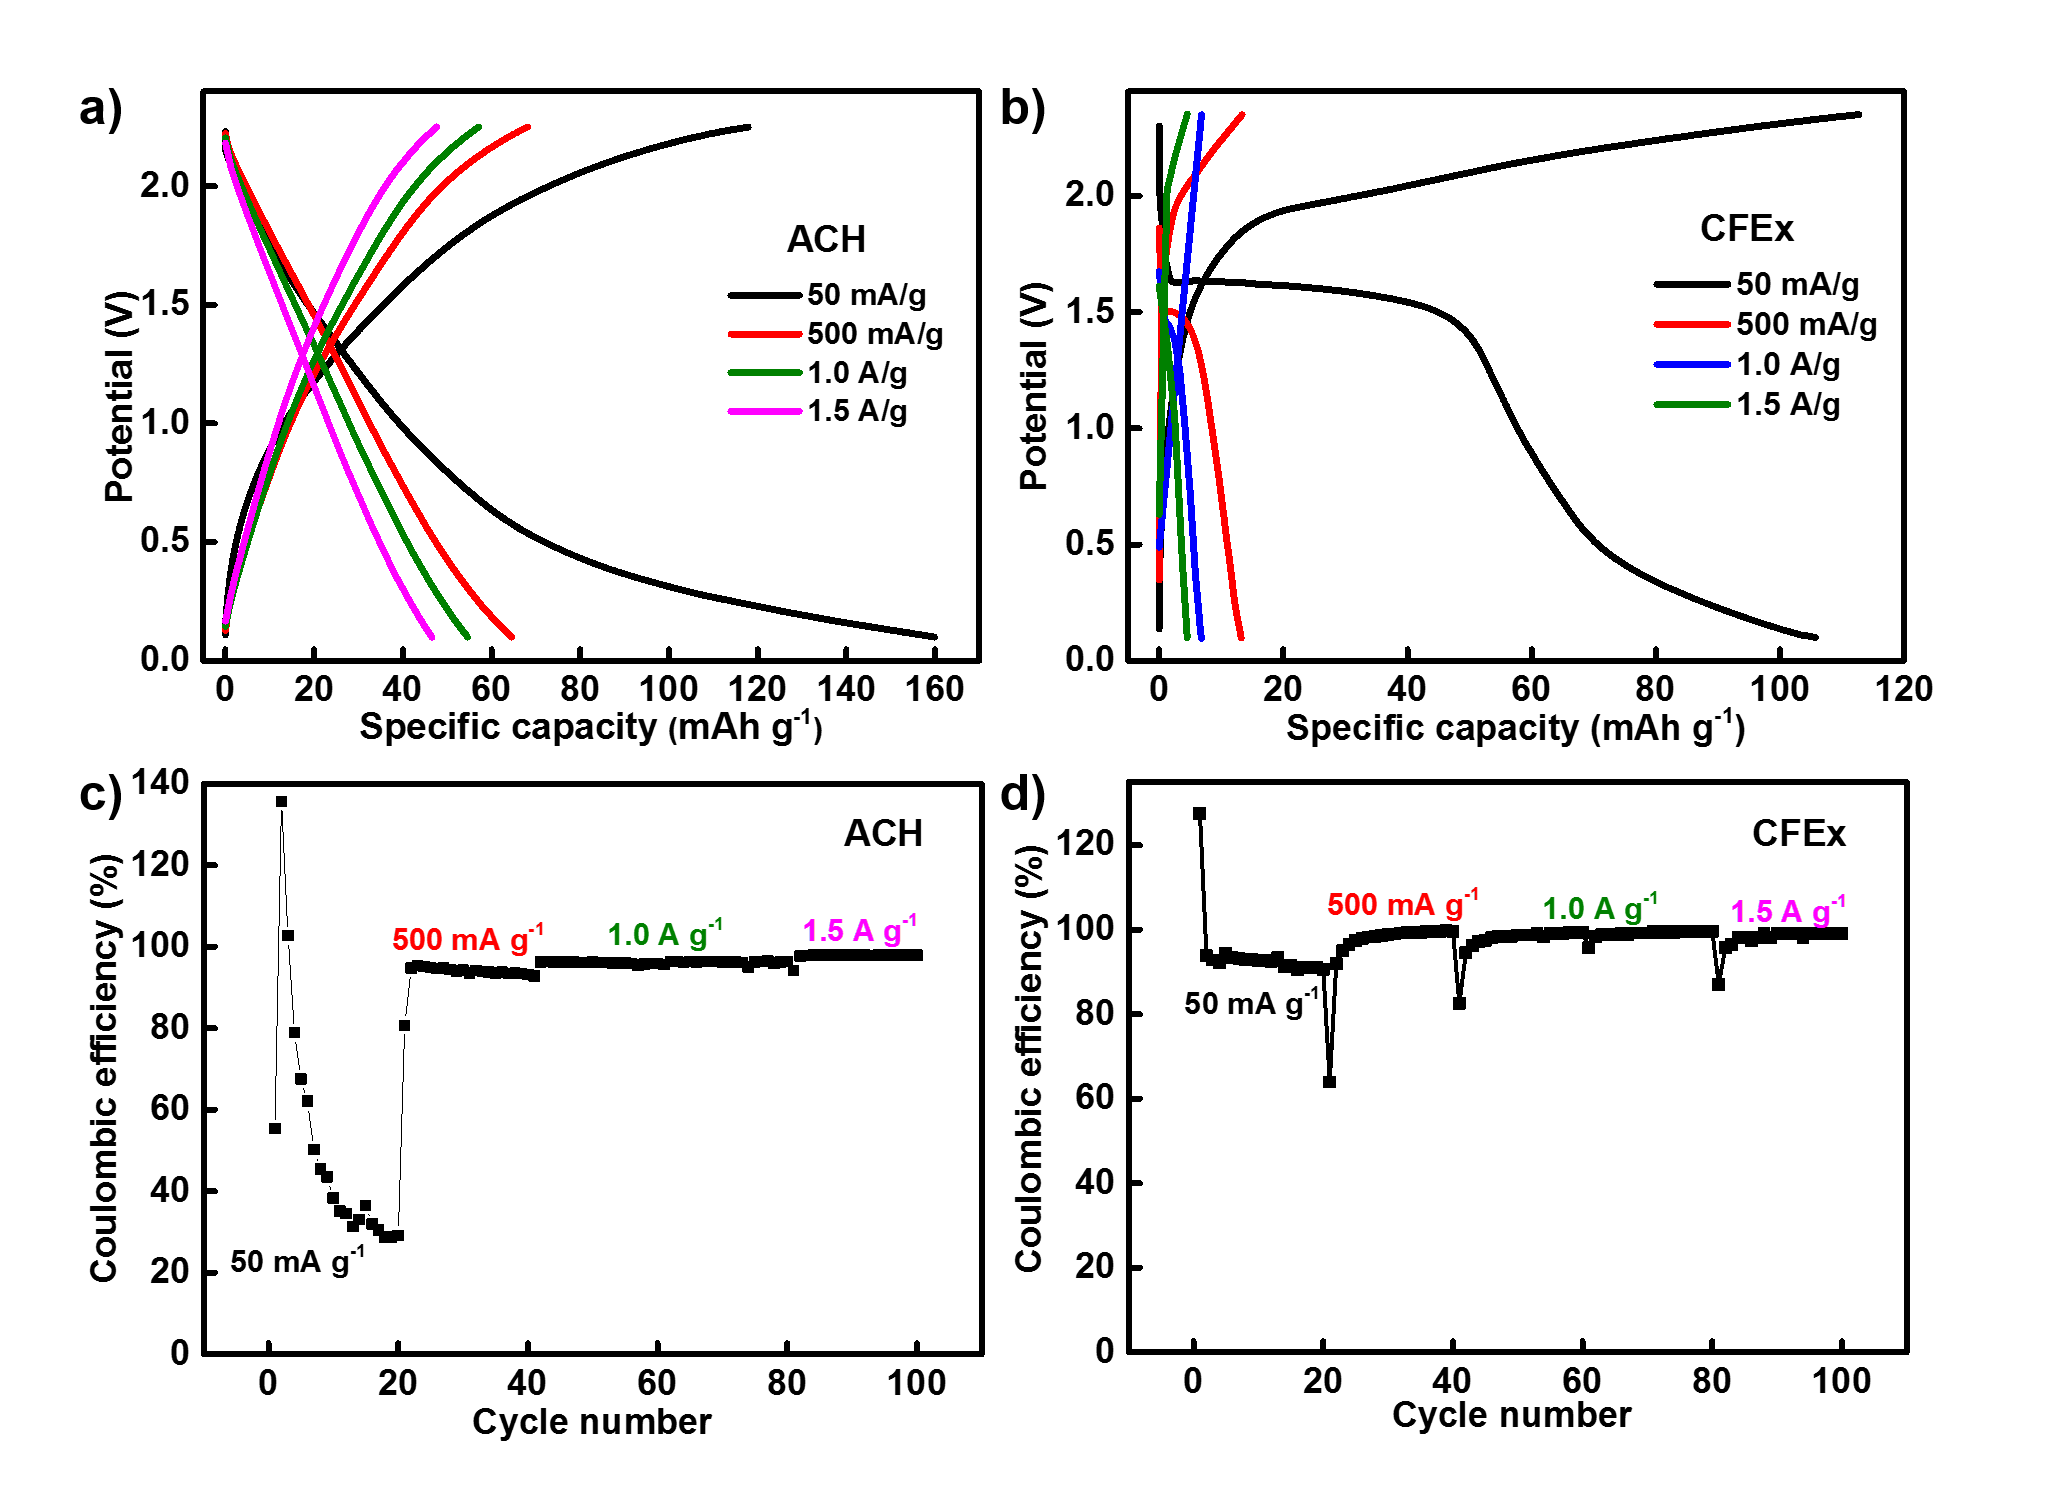
\includegraphics[width=\textwidth]{Figures/chap5fig/cfexachlong.png}
    \caption{Discharge capacities of a) ACH and b) CFEx cathodes at current rates of 50mAg$^{-1}$, 500mAg$^{-1}$, 1.0 Ag$^{-1}$ and 1.5 Ag$^{-1}$ along with their coulombic efficiencies. }
  \label{Figures/chap5fig:cfexachlong}
\end{figure}

\newpage
% Are the following the conclusions?
\section{Conclusion}
In summary, AC derived from human hair proved to be the best carbon-based cathode among all the tested materials in this work, with a specific capacity of 100 mAh g$^{-1}$ at a potential of 1.9 V with a coulombic efficiency of $\sim$90$\%$. Intercalation and deintercalation of \ce{AlCl4-} takes place in the very few graphitic layers. We found that in CFEx \ce{AlCl4-} anions seep in and out of the gaps in between the fullerenes changing its structure and slightly expanding the crystal lattice during charging(Figure \ref{Figures/chap5fig:cfexmech}). Moreover, fullerenes maintain their structural integrity and coulombic efficiency throughout the cycles. Hemp fibers and Super-P on the other hand, have a highly amorphous structure, which degraded after every cycle, resulting in a low capacity value. Figure \ref{Figures/chap5fig:cfexachlong} compares the 50th cycle measurement for Al/hair and Al/natural graphite cell. It not only displays a higher specific capacity than conventional graphite, but also a high battery voltage of 1.92 V with an energy density of 202 Wh kg$^{-1}$. The high battery performance can be attributed to the porosity of the material combined with high surface area and hetero-atom doping effects, combining surface-based non-Faradaic and Faradaic contributions. Hair based aluminium-ion batteries would not only be cheaper than state of the art, but would also be one of its kind bio-degradable materials in the battery industry. 



